\documentclass[runningheads,oribibl,]{article}

\newif\ifincludeproofs
\newif\iffinal
\finaltrue


\usepackage{calc}
\usepackage{ifthen}
\usepackage[utf8]{inputenc}
\usepackage{xspace}
\usepackage{amsmath, amssymb, latexsym, amsfonts}
\usepackage[only, lightning, llbracket, rrbracket]{stmaryrd}
\usepackage{enumerate}
\usepackage{multirow}
\usepackage{rotating}
\usepackage{thmtools,thm-restate}


\usepackage[hypertexnames=true,
            plainpages=false,
            linktocpage=false,
            breaklinks=true,
            pdfpagelabels=true,
            pageanchor=true,
            bookmarks=false,
            pdftex,
            final,
            verbose=false,
            debug=false,
            a4paper,
            naturalnames=false,
                        hyperindex=true]{hyperref}

\hypersetup{
         pdftitle={},
         pdfauthor={},
         pdfsubject={},
         pdfkeywords={},
         pdfcreator={pdfLaTeX},
         pdfpagemode=None,
         colorlinks,
         anchorcolor=black,
         citecolor=black,
         filecolor=black,
         linkcolor=black,
         urlcolor=black,
                  pdftex}
\pdfcompresslevel=9

\pagestyle{plain}
\bibliographystyle{plain}

\usepackage{graphicx}
\usepackage{tikz}
\usetikzlibrary{matrix,calc,positioning,fit,arrows,decorations.markings,decorations.pathmorphing,backgrounds,automata,shapes.symbols,shapes.arrows,shapes.geometric,shapes.callouts,decorations.pathreplacing,decorations.markings,decorations.pathmorphing,decorations.text}




\usepackage[final]{listings}

\definecolor{darkviolet}{rgb}{0.5,0,0.4}
\definecolor{darkgreen}{rgb}{0,0.4,0.2}
\definecolor{darkblue}{rgb}{0.1,0.1,0.9}
\definecolor{darkgrey}{rgb}{0.5,0.5,0.5}
\definecolor{lightblue}{rgb}{0.4,0.4,1}
\lstdefinestyle{eclipsish}{
    basicstyle=\scriptsize\ttfamily,
    emphstyle=\color{red}\bfseries,
    keywordstyle=\color{darkgreen}\bfseries,
    keywordstyle=[2]\color{darkviolet}\bfseries,
    commentstyle=\color{darkgrey},
    stringstyle=\color{darkblue},
    numberstyle=\color{darkgrey}\ttfamily\tiny,
    emphstyle=\color{red},
        morecomment=[s][\color{lightblue}]{/**}{*/},
     showstringspaces=false,
  numbers=left,
  numbersep=5pt,
  xleftmargin=2.5ex,
  xrightmargin=2.4ex,
  breakindent=3ex,
  breakautoindent,
  numberblanklines=false,
  escapeinside={(*@}{@*)},
  mathescape=true,
}

\lstdefinelanguage{GCD}[]{C}
  {morekeywords=[2]{write, read,dispatch\_s, dispatch\_a,forkjoin,c\_queue, s\_queue, sleep, apply,require,?,!,??,!!},   alsoletter={^},   morekeywords= {def,foreach,block, ^,string,bool, global,  elseif,
   group,select,with,where,in, wait}
  }\lstset{language=GCD,style=eclipsish}






\newcommand{\mleq}{\preceq}
\newcommand{\tuple}[1]{\langle#1\rangle\xspace}
\newcommand{\set}[2]{\left\{#1\,\vert\,#2\right\}}
\newcommand{\veve}[1]{\ensuremath{\left| #1 \right|}}
\newcommand{\size}[1]{\veve{#1}}
\newcommand{\iarr}{\ding{234}\xspace} \newcommand{\act}[1]{\stackrel{\smash{{\tiny #1}}}{\Longrightarrow}}

\newcommand{\Aa}{\ensuremath{\mathcal{A}}\xspace}
\newcommand{\Bb}{\ensuremath{\mathcal{B}}\xspace}
\newcommand{\Cc}{\ensuremath{\mathcal{C}}\xspace}
\newcommand{\Dd}{\ensuremath{\mathcal{D}}\xspace}
\newcommand{\Ff}{\ensuremath{\mathcal{F}}\xspace}
\newcommand{\Ll}{\ensuremath{\mathcal{L}}\xspace}
\newcommand{\Pp}{\ensuremath{\mathcal{P}}\xspace}
\newcommand{\Qq}{\ensuremath{\mathcal{Q}}\xspace}
\newcommand{\Ss}{\ensuremath{\mathcal{S}}\xspace}
\newcommand{\Tt}{\ensuremath{\mathcal{T}}\xspace}
\newcommand{\Ts}{\ensuremath{\mathcal{TS}}\xspace}
\newcommand{\Xx}{\ensuremath{\mathcal{X}}\xspace}
\newcommand{\Gg}{\ensuremath{\mathcal{G}}\xspace}
\newcommand{\Vv}{\ensuremath{\mathcal{V}}\xspace}

\newcommand{\e}{\ensuremath{\varepsilon}\xspace}

\newcommand{\mbar}{\ensuremath{\overline{m}}\xspace}

\newcommand{\BB}{\ensuremath{\mathbb{B}}\xspace}
\newcommand{\DD}{\ensuremath{\mathbb{D}}\xspace}
\newcommand{\NN}{\ensuremath{\mathbb{N}}\xspace}
\newcommand{\ZZ}{\ensuremath{\mathbb{Z}}\xspace}

\newcommand{\cfg}{\ensuremath{\mathcal{CFG}}\xspace}

\newcommand{\sem}[1]{\ensuremath{\llbracket #1 \rrbracket}}
\newcommand{\pow}[1]{\ensuremath{2^{#1}}}


\newcommand{\cfont}[1]{\ensuremath{\mathtt{#1}}\xspace}
\DeclareMathOperator{\dotcup}{\mathaccent\cdot\cup}
\DeclareMathOperator{\bigdotcup}{\ooalign{\cr\hfill\hfill}}
\DeclareMathOperator{\passert}{\cfont{assert}}
\DeclareMathOperator{\nassert}{\cfont{nassert}}
\DeclareMathOperator{\inverse}{\cfont{inverse}}
\DeclareMathOperator{\predset}{\cfont{set}}
\newcommand{\main}{\ensuremath{\textit{main}}\xspace}
\DeclareMathOperator{\incr}{\cfont{incr}}
\DeclareMathOperator{\decr}{\cfont{decr}}
\DeclareMathOperator{\zerotest}{\cfont{is\_zero}}
\DeclareMathOperator{\ack}{\cfont{ack}}

\newcommand{\dsqsseq}{\mathaccent\cdot\sqsubseteq}



\newcommand{\eqzero}{\ensuremath{\smash{\stackrel{\text{\tiny ?}}{=}}0}}

\newcommand{\CQID}{CQID\xspace}
\newcommand{\SQID}{SQID\xspace}
\newcommand{\QID}{QID\xspace}
\newcommand{\GID}{GID\xspace}
\newcommand{\dep}{\ensuremath{\diamond}\xspace}


\newcommand{\lts}{\textsc{Lts}\xspace}
\newcommand{\pds}{\textsc{Pds}\xspace}
\newcommand{\mpds}{\textsc{Mpds}\xspace}
\newcommand{\petri}{\textsc{Pn}\xspace}
\newcommand{\pn}{\textsc{Pn}\xspace}
\renewcommand{\gcd}{\textsc{Gcd}\xspace}
\newcommand{\qdas}{\textsc{Qdas}\xspace}
\newcommand{\pqdas}{\textsc{pQdas}\xspace}
\newcommand{\eqdas}{\textsc{eQdas}\xspace}
\newcommand{\twocs}{2\textsc{Cs}\xspace}

\newcommand{\fifo}{fifo\xspace}
\newcommand{\dexpspace}{\textsc{ExpSpace}\xspace}
\newcommand{\dexpspacecomplete}{\textsc{ExpSpace-C}\xspace}
\newcommand{\pspace}{\textsc{PSpace}\xspace}
\newcommand{\pspacecomplete}{\textsc{PSpace-C}\xspace}
\newcommand{\ptime}{\textsc{PTime}\xspace}
\newcommand{\ptimecomplete}{\textsc{PTime-C}\xspace}
\newcommand{\nlogspace}{\textsc{NLogSpace}\xspace}
\newcommand{\dexptime}{\textsc{ExpTime}\xspace}
\newcommand{\dexptimecomplete}{\textsc{ExpTime-C}\xspace}


\newcommand{\QDAS}{\ensuremath{\tuple{\CQID, \emptyset,\allowbreak \Gamma,
\allowbreak \mathtt{main},\allowbreak \Xx,\allowbreak \Sigma,\allowbreak
(\Ts_\gamma)_{\gamma\in\Gamma}}}}
\DeclareMathOperator{\Reach}{\textit{Reach}}

\newcommand{\Param}{\ensuremath{\mathcal{I}}}
\newcommand{\PEval}{\ensuremath{\mathbf{e}}}

\newcommand{\Cover}{\ensuremath{\textit{Cover}}}
\newcommand{\Reachloss}{\Cover}


\newcommand{\SSigma}{\ensuremath{\smash{\widetilde{\Sigma}}}}

\newcommand{\istate}{\ensuremath{s^0}}

\newcommand{\Graph}{\ensuremath{G}}
\newcommand{\Data}{\ensuremath{\vec{d}}}
\newcommand{\DData}{\ensuremath{\widehat{\vec{d}}}}

\newcommand{\queue}{\ensuremath{\textit{queue}}}
\newcommand{\state}{\ensuremath{\textit{state}}}
\newcommand{\head}{\ensuremath{\textit{head}}}
\newcommand{\tail}{\ensuremath{\textit{tail}}}
\newcommand{\enqueue}{\ensuremath{\textsf{enqueue}}}
\newcommand{\dequeue}{\ensuremath{\textsf{dequeue}}}
\newcommand{\step}{\ensuremath{\textsf{step}}}
\newcommand{\letwait}{\ensuremath{\textsf{letwait}}}
\newcommand{\terminate}{\ensuremath{\textit{terminate}}}
\newcommand{\ctg}{\ensuremath{\textsc{Ctg}}\xspace}
\newcommand{\disps}{\ensuremath{\cfont{dispatch_s}}}
\newcommand{\dispa}{\ensuremath{\cfont{dispatch_a}}}
\newcommand{\forkjoin}{\ensuremath{\cfont{forkjoin}}\xspace}
\newcommand{\guardson}[1]{\ensuremath{\mathsf{guards}\left(#1\right)}}
\newcommand{\valof}[1]{\ensuremath{\mathsf{vals}\left(#1\right)}}
\newcommand{\assignon}[1]{\ensuremath{\mathsf{assign}\left(#1\right)}}
\newcommand{\Parikh}{\ensuremath{\mathsf{Parikh}}}
\newcommand{\mystate}[2]{\ensuremath{s^{#1}_{\mathtt{#2}}}}

\newcommand{\push}{\ensuremath{\cfont{push}}}
\newcommand{\pop}{\ensuremath{\cfont{pop}}}
\newcommand{\emptystack}{\ensuremath{\cfont{empty?}}}

\newcommand{\ko}{\ensuremath{\lightning}}
\newcommand{\ok}{\ensuremath{\checkmark}}

\newcommand{\vstrut}[1]{\rule{0pt}{#1}}

\newcommand{\inputproof}[1]{\ifincludeproofs\else\fi}

\newenvironment{myitemize}{\begin{list}{\labelitemi}{\setlength{\topsep}{4pt}\setlength{\partopsep}{0pt}
\setlength{\itemsep}{0pt}
\setlength{\itemindent}{0ex}
\setlength{\listparindent}{0ex}
\setlength{\leftmargin}{4ex}\setlength{\labelwidth}{2ex}
}}
{\end{list}}

\tikzstyle{state}=[draw,ellipse,inner sep=1pt,minimum size=2.5ex,font=\small]
\tikzstyle{box}=[state,rectangle,minimum size=2.3ex]
\tikzstyle{lop}=[->,looseness=5,out=30,in=-30,inner sep=1pt,shorten >=1pt]
\tikzstyle{lab}=[font=\tiny]
\tikzstyle{na}=[baseline=-0.5ex]


\def\eor{\ifmmode\squareforqed\else{\unskip\nobreak\hfil
\penalty50\hskip1em\null\nobreak\hfil
\parfillskip=0pt\finalhyphendemerits=0\endgraf}\fi}


\newtheorem{theorem}{Theorem}{}
\newtheorem{proposition}{Proposition}{}
\newtheorem{lemma}{Lemma}{}
\newtheorem{corollary}{Corollary}{}
\newtheorem{example}{Example}{}
\newenvironment{proof}{\noindent{\it Proof.\hspace*{.5cm}}}{}
\newcommand{\qed}{\hfill}




\newcommand\fixme[1]{}
\newcommand\detail[1]{}
\newcommand\change[1]{}
\newcommand\afaire[1]{}


\begin{document}
\title{Queue-Dispatch Asynchronous Systems}
\author{Gilles Geeraerts
\and Alexander Heußner
\and Jean-François Raskin\1.5ex]
    \multicolumn{2}{c|}{}& concurrent & serial & both\\
    \cline{1-5}
    \multirow{3}{*}{\begin{sideways}{dispatch\ \ }\end{sideways}}      \hspace{1ex}\vstrut{3ex}
    &synchr.  & \dexptimecomplete & \ \ \ \pspacecomplete\ \ \  & \dexptimecomplete\1.5ex]
    &both  & \ko & (\ko) & (\ko)\\
  \end{tabular}}
                                            \0.5ex]@*)
block increase():
  count = count + 1 (*@\label{lst:count}\0.5ex]@*)
def main():
  // read input matrix1, matrix2
  count = 0
  for i in range(l):  (*@\label{lst:fork-start}@*)
    for j in range(n):
      dispatch_a(workqueue,one_cell(i,j))
  wait(count = l*n)  (*@\label{lst:join}@*)
  // print the result
  \end{lstlisting}
  \caption{\gcd(-like) program for parallel matrix multiplication}
\label{fig:example-gcd}
\end{figure}


\paragraph{\bf Basic Notations:} Given a set , let  denote its
cardinality. For an -indexed family of sets , we
write elements of  in bold face, i.e.,
. The -component of  is
written , and we identify  with the indexed
family of elements .
We use  to denote the disjoint union of sets.
An \emph{alphabet}  is a finite set of \emph{letters}. We
write  for the set of all \emph{finite words}, over 
and denote the empty word by . The concatenation of two
words  is represented by . For a letter
 and a word , let  be
the number of occurrences of  in .
We use standard complexity classes, e.g., polynomial time
(\ptime) or deterministic exponential time (\dexptime), and mark
completeness by appending ``-C'' (\pspacecomplete).

Let  be a finite \emph{\bf data domain}
with an \emph{initial element} , and let  be a finite
set of variables ranging over . A \emph{valuation} of the
variables in  is a function .  An
\emph{atom} is an expression of the form  or , where
 and . A \emph{guard} if a finite conjunction of
atoms. An assignment is an expression of the form , where
 and . Let ,  and
 denote respectively the sets of all guards, assignments
and valuations over variables from . Guards, atoms and valuations
have their usual semantics: for all valuations  of  and all
, we write  iff  satisfies
.


\smallskip\noindent A \emph{\bf pushdown system with data} is a
pushdown system (see~\cite{bouajjani-a-1997-135-a} for details)
equipped with a finite set of variables  over a
finite domain . A configuration of a \pds with data is a pair
 where  is a control state,  is the stack content,
and  is a valuation of the variables

\begin{restatable}{proposition}{propreachpdsdata}\label{prop:reach_pds_data}
  The reachability problem is \dexptimecomplete for \pds with data.
\end{restatable}


\smallskip\noindent A \emph{\bf Petri net} (\petri) is a tuple
 where  is a finite set of places, a
\emph{marking} of the places is function  that
associates, to each place  a number  of tokens,  is
finite set of transitions, each transition  is a pair  where
           and  are respectively the \emph{input} and
\emph{output functions} of , and  is the \emph{initial
  marking}. Given two markings  and , we let 
iff  for all . Given a marking , a
transition  is \emph{enabled} in  iff  for all . When  is enabled in , one can
\emph{fire} the transition  in , which produces a new marking
 s.t.  for all . This is denoted
\smash{}, or simply  when the
transition identity is irrelevant.  A \emph{run} is a finite sequence
 s.t. for all : .  For a \petri , we denote by  (resp. )
the \emph{reachability (coverability) set} of , i.e. the set of all
markings  s.t. there exists a run  of  with
 (). The \emph{coverability problem} asks, given a
\petri  and a marking , whether . It is
\dexpspace-complete~\cite{esparza-j-1998-374-a}. The termination
problem, i.e., whether all executions of the Petri net
are finite, is decidable in \dexpspacecomplete~\cite{lipton,rackoff}.






\section{Queue-dispatch asynchronous systems}

\paragraph{\bf Syntax:} We now define our formal model for
queue-dispatch asynchronous systems.
Let  be a finite data domain containing an \emph{initial value}
. A \emph{queue-dispatch asynchronous system} (\qdas)  is
a tuple  where:
\begin{myitemize}
  \item  and  are respectively sets of
    \emph{(c)oncurrent} and \emph{(s)erial queues};
  \item  is the finite set of \emph{blocks} and
     the \emph{initial block}.  Each block
     is a tuple  where  is an \lts and
     a distinct final state;
  \item  is a finite set of -valued variables;
  \item  is the set of \emph{actions}, with
    \linebreak[1] .
\end{myitemize}

We assume that , and all  for
 are disjoint from each other. Let
,
,
, and
 (where ).
We further assume that .

\paragraph{\bf Call-task graphs:}
We formalize the semantics of \qdas using the notion of
\emph{call-task graph} (\ctg) to describe the system's global
configurations.

A configuration of a \qdas (see Fig.\,\ref{fig:example-ctg} for an
example) contains a set of running tasks, represented by \emph{task
  vertices} (depicted by round nodes), a set of called but unscheduled
blocks, represented by \emph{call vertices} (square nodes). Call
vertices are held by queues, and the linear order of each queue is
represented by \emph{queue edges} (solid edges). Synchronous calls add
an additional dependency (the caller is waiting for the termination of
the callee) that is represented by a \emph{wait edge} (dashed edges)
between the caller and the callee. Wait edges are also inserted
between the head of a \emph{serial} queue and the running task that
has been extracted from this queue (if it exists) to indicate that the
task has to terminate before a new block can be dequeued.  Note that
only vertices without outgoing edges can execute a computation step,
the others are currently blocked.  Each node  is labeled by a block
, an by the identifier  of the queue that
contains it (for call vertices) or that contained it (for task
vertices). Task vertices are labeled by their current state
 (for convenience, we also label call vertices by the
initial state of their respective blocks -- not shown in the figure).



\vspace{-1ex}
\begin{example}
  The \ctg in Fig.\,\ref{fig:example-ctg} depicts a configuration of a
  \qdas with two queues. Queue  is serial (note the outgoing wait
  edge to the running task) and contains ,
  and  is parallel with content . There are 4
  active tasks, two of them (\texttt{main} and the task running
  ) are blocked. The task running  has been
  dequeued from  and is currently at location . \eor
\end{example}
\vspace{-1ex}

\begin{figure}[t]
    \centering
        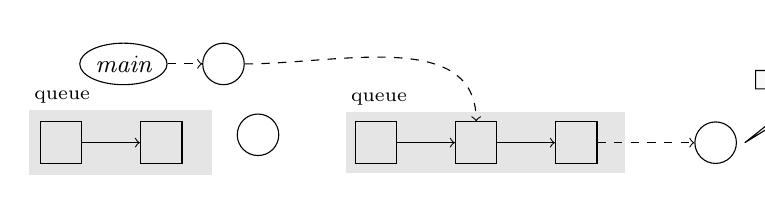
\begin{tikzpicture}
  [zstd/.style={state,font=\small,inner sep=1pt,minimum size=15pt},
  zstd2/.style={zstd,rectangle},
  lab/.style={font=\tiny,inner sep=1pt},
  anchor=west]

  \draw (0,0) node[zstd2] (00) {};
    \draw (00.south east) node[lab,anchor=south west] {};
  \draw (00)+(1,0) node[zstd2] (01) {};
    \draw (01.south east) node[lab,anchor=south west] {};
  \draw (00) edge[->] (01);

  \draw (4,0) node[zstd2] (10) {};
    \draw (10.south east) node[lab,anchor=south west] {};
  \draw (10)+(1,0) node[zstd2] (11) {};
    \draw (11.south east) node[lab,anchor=south west] {};
  \draw (11)+(1,0) node[zstd2] (12) {};
    \draw (12.south east) node[lab,anchor=south west] {};
  \foreach \x / \y in {10/11,11/12}
    \draw (\x) edge[->] (\y);

  \draw (12)+(1.5,0) node[zstd] (13) {};
    \draw (13.south east) node[lab,anchor=north west] {};
    \draw (13.north east) node[lab,anchor=south west] {};
  \draw[dashed] (12) edge[->] (13);

  \draw (0.5,1) node[zstd] (main) {\main};
    \draw (main.south east) node[lab,anchor=north west] {};
    \draw (main.north east) node[lab,anchor=south west] {};
  \draw (main)+(1,0) node[zstd] (one) {};
    \draw (one.south east) node[lab,anchor=north west] {};
    \draw (one.north east) node[lab,anchor=south west] {};
  \draw[dashed]
        (main) edge[->] (one)
        (one) edge[->,out=0,in=90] (11);

  \draw (2.5,0.1) node[zstd] (two) {};
    \draw (two.south east) node[lab,anchor=north west] {};
    \draw (two.north east) node[lab,anchor=south west] {};


    \begin{pgfonlayer}{background}
      \path (01)+(0.5,0)  coordinate (dummy);
      \draw node[fit=(00) (01) (dummy),fill=gray!20,inner sep=4pt] (c1) {};
      \draw (c1.north west)
        node[anchor=south west,inner sep=2pt,font=\scriptsize]
        {queue };
      \path (12)+(0.5,0)  coordinate (dummy);
      \draw node[fit=(10) (12) (dummy),fill=gray!20] (c1) {};
      \draw (c1.north west)
        node[anchor=south west,inner sep=2pt,font=\scriptsize]
        {queue };
    \end{pgfonlayer}

  \draw[overlay]
  (13) +(0.5,0.8) node[draw,
  rectangle callout,callout absolute pointer={(13.east)+(0.1,0)},font=\scriptsize,
    fill=gray!5,text width=1.8cm, align=center]
  {  };
\end{tikzpicture}
\caption{\ctg for a \qdas with a concurrent queue  and  a serial queue
    \label{fig:example-ctg}}
    \vspace{-3ex}
  \end{figure}


  Formally, given a \qdas , a \emph{call-task
    graph} over  is a tuple
   where:  is a finite set of \emph{vertices}, partitioned into a set
   of \emph{call vertices} and a set  of \emph{task
    vertices};  is a set of \emph{edges};
   labels each vertex by a block;
   associates each vertex to
  a queue  identifier
  (or ); and  associates each vertex
  to a \lts state.
  For each , let . The set
   is partitioned into the set  of \emph{wait edges} and the
  set  of \emph{queue edges} where, for
  each , .

A \ctg is \emph{empty} iff . The \emph{Parikh image}
 of a \ctg  of  is a function
, s.t. for all : . Given two Parikh images  and
, we let  iff for all : .
A \emph{path} (of length ) in  is a sequence of
vertices  s.t. for all :
. Such a path is \emph{simple} iff 
for all . The \emph{restriction} of  to
 is the \ctg , where , and ,
 and  are respectively the restrictions of
,  and  to .

In the rest of the paper, we  assume that all the \ctg we
consider are \emph{well-formed}, i.e., they fulfill the following
requirements:
\begin{enumerate}
  \item For each : 
    where  are the states of .
\item Each \emph{call} vertex has at most one outgoing (queue or wait)
  edge, at most one incoming \emph{wait} edge, and at most one
  incoming \emph{queue} edge. Each \emph{task} vertex has at most one
  outgoing, and at most one incoming \emph{wait} edge.
\item For each , the restriction of  to 
  is either empty or contains one and only one simple path of length
  . Intuitively, this ensures the well-formedness of the
  queues.
\item For each , there is at most one task vertex 
  s.t. . This ensures that queues in  indeed
  force the serial execution of its members.
\end{enumerate}

For convenience, we also introduce the following notations. Let
 be a \ctg, and let  be a queue identifier of
. Then,  and  denote
respectively the head and the tail of  in the configuration
described by , that is,  is the call
vertex  that has no incoming queue edge, or , if such
a vertex does not exist; and  is the call vertex
 that has no outgoing \emph{queue} edge (but possibly an
outgoing \emph{wait} edge), or , if such a vertex does not
exist. Remark that, when they exist, these vertices are necessarily
unique because of the well-formedness assumptions. Finally, we say
that a vertex  is \emph{unblocked} iff it has no outgoing edge, and
that it is \emph{final} iff   is an \emph{unblocked task}
vertex and   (that is,  represents a
task that has reached the final state of its transition system and is
not waiting on another task).





Let us now define several operations on \ctg. We will rely on these
operations when defining the formal semantics of \qdas. Let  be a
\qdas and 
be a \ctg for . Then:
\begin{myitemize}
\item for all :  is the restriction of
   to .
\item for all  and ,
   is the \ctg  where: ,  is a
  fresh queue vertex, , ,
  , and for all :
   and .  Finally,
  , where: 
   if
  ,
  and  otherwise, and  if  is a
  \emph{task} node s.t. , then ,
  otherwise . Intuitively, this operation inserts a
  call to  in the queue , by creating a new vertex  and
  adding an edge to maintain the FIFO ordering, if necessary (set
  ). In the case of a \emph{serial} queue that was empty before
  the enqueue, a supplementary edge (in set ) might be necessary
  to ensure that  is blocked by a currently running  which has
  been extracted from .
\item for all , if  is different from  and
  \emph{unblocked}, then  is the \ctg
   where
   and
  . Otherwise,  and
   is undefined. Intuitively, this operation
  removes the first (with respect to the FIFO ordering) block from 
  and turns the corresponding \emph{call} vertex  into a
  \emph{task} vertex, meaning that the block is now running as a
  task.\item for all , 
  is a \emph{set} of \ctg defined as follows.  iff there exists an
  \emph{unblocked}  s.t. ,  and
  for all : . Remark that
   can be empty. Intuitively, each graph in
   corresponds to the firing of an
  -labeled transition by a task that is not blocked.
\item for all unblocked , all :
   is either the \ctg  if
  , or the \ctg  if . Intuitively, this operation adds a wait
  edge between nodes  and  when , and does not
  modify the \ctg otherwise.
\end{myitemize}

\paragraph{\bf Semantics of \qdas:} For a \qdas  with set of variables
, a \emph{configuration} is a pair , where
 is a \ctg of  and .  The
operational semantics of  is given as a transition system
 whose states are configurations of ; and whose
transitions reflect the semantics of the actions labeling the
transitions of the \qdas. Formally, given a \qdas ,
 is the labeled transition system  where:   contains all the pairs
 where , and  is a \ctg
of ,   with  for
all , and , where  is a \emph{task node},
,  and
,   and 
 iff
one of the following holds:
\begin{description}
\item[Async. dispatch:] , , and
  there are  and
   s.t.:
  .
\item[Sync. dispatch:] ,  and there
  are  and
  
  s.t.: 
  where  is the node whose  has changed during the 
  operation, and  is the fresh node that has been created by the
   operation. That is, a queue vertex  labeled by
   is added to  and a \emph{wait} edge is added between the
  node  representing the task that performs the \emph{synchronous}
  dispatch, and , as the dispatch is \emph{synchronous}.
\item[Test:] , , ,
  and there is  s.t.
  .
\item[Assignment:] , , for
  all :  and there is
  
  s.t. .
\item[Scheduler action:] ,  and:
  \begin{itemize}
  \item either there is a final vertex 
    s.t. ;
  \item or there is  s.t.  and
    . That is, the scheduler schedules a
    block (represented by ) from a concurrent queue.
  \item or there is  s.t.  ,  is
    \emph{unblocked}, as well as  and
    . That is, the scheduler schedules a
    block (represented by ) from the serial queue . As the queue
    is serial, a \emph{wait} edge is inserted between the next waiting
    block in  (now represented by ) and .
  \end{itemize}

 \end{description}


 A \emph{run}  of a \qdas is an alternating sequence  of configurations and actions where
  for all  and
 . A run is \emph{finite} if this sequence is
 finite.
 A configuration  is \emph{reachable} in  iff there
 exists a finite run  of  s.t. . We
 denote by  the set of all reachable configurations
 of~.

 The decision problem on \qdas we mainly consider in this work is the
 \emph{Parikh coverability problem}: given a \qdas  with set of
 locations  and a function , it asks whether
 there is 
 s.t. . When the answer to this question is `yes',
 we say that  is \emph{Parikh-coverable} in . It is well-known
 that meaningful verification questions can be reduced to this
 problem. For instance, consider a \emph{mutual exclusion} question,
 asking whether it is possible to reach, in a \qdas , a
 configuration in which at least two tasks are executing the same
 block  and are in the same control state . If yes, the
 mutual exclusion (of control state ) is violated. This can be
 encoded into an instance of the Parikh coverability problem, where
  and  for all , and would allow,
 for example, to verify if there are more than one block of type
 \texttt{increase} running in
 Example\,\ref{ex:gcd-matrixmult}.

 In addition, we look at the \emph{(universal) termination problem}:
 given a \qdas , it asks whether all executions of  are
 finite, i.e., there is no infinite run of .
 Regarding Example\,\ref{ex:gcd-matrixmult}, this
 permits to test whether the \texttt{main} task terminates, i.e.,
 all dispatched blocks terminate.



\section{From the Parikh coverability problem to Termination\label{sec:parikh-cover-probl}}

Before regarding the termination problem, we first study
in this section the Parikh coverability problem from a
computational point of view. As expected, this problem is undecidable
in general. However, when restricting the types of queues and
dispatches that are allowed, it is possible to retain decidability. In
these cases, we characterize the complexity of the problem. Formally,
we consider the following subclasses of \qdas. A \qdas  with set
of transitions , set of serial queues  and set of
concurrent queues , is \emph{synchronous} iff there exists no
 with ; it is \emph{asynchronous} iff there exists no
 with ; it is \emph{concurrent} iff  and
; it is \emph{serial} iff  and
; it is \emph{queueless} iff
.


\paragraph{\bf Queueless \qdas:} In a queueless \qdas, there is no dispatch
possible, so the only task that can execute at all time is the
\texttt{main} one. Thus, configurations of queueless \qdas can be
encoded as tuples , where  is a state of
\texttt{main}, and  is a valuation of the variables.
Hence queueless \qdas are essentially \lts with variables over
a finite data domain, thus:
\begin{proposition}\label{prop:queueless}
  The Parikh coverability is \pspacecomplete
  for queueless \qdas.
\end{proposition}

\paragraph{\bf Synchronous \qdas:}

\begin{figure}[!t]
  \centering(a)
  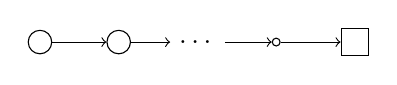
\begin{tikzpicture}[baseline=-0.5ex,every node/.style={inner sep=3pt}]
    \foreach \x / \z in {0/0,1/1}
      \draw(1*\x,0) node[circle,draw] (\x) {\tiny{}};
    \draw (2,0) node (2) {\dots};
    \draw(3,0) node[circle,draw,inner sep=1pt] (3) {\tiny{}};
    \draw(4,0) node[rectangle,inner sep=5pt,draw] (4) {\tiny{}};
    \foreach \x / \y in {0/1,1/2,2/3,3/4}
    \draw (\x) edge [->] (\y);
  \end{tikzpicture}\hspace*{1cm}(b)
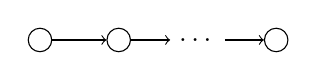
\begin{tikzpicture}[baseline=-0.5ex,every node/.style={inner sep=3pt}]
    \foreach \x / \z in {0/0,1/1}
      \draw(1*\x,0) node[circle,draw] (\x) {\tiny{}};
    \draw(3,0) node[circle,draw] (3) {\tiny{}};
    \draw (1*2,0) node (2) {\dots};
    \foreach \x / \y in {0/1,1/2,2/3}
    \draw (\x) edge [->] (\y);
  \end{tikzpicture}
  \caption{The two possible forms of reachable {\ctg}s in a synchronous \qdas}
  \label{fig:config-sync}
\end{figure}


In synchronous \qdas, there is no concurrency in the sense there is at
most one running task that can fire an action at all times. All the
other tasks have necessarily performed a \emph{synchronous} dispatch
and are thus blocked. More precisely, in every reachable configuration
 of a synchronous \qdas,  is of one of the
forms depicted in Fig.~\ref{fig:config-sync}
(i.e.  and either  or ). When the current \ctg is of the form
Fig.~\ref{fig:config-sync}(a), the only possible action is that the
scheduler starts running 's block and we obtain a graph of the
form Fig.~\ref{fig:config-sync}(b). In the case where the \ctg is of
the form (a), either  terminates, which removes  from the
\ctg, or  executes an internal action, which does not change the
shape of the \ctg, or  does a synchronous call, which adds a call
vertex as successor of  which will be directly
scheduled. W.l.o.g., we assume in the following that for synchronous
\qdas the combined action of \disps and scheduling the dispatched
block is atomic.



                                For a \ctg  and , we write
  iff for all :
 and the empty \ctg is mapped to the empty word .
Given a synchronous \qdas  with set of local
states  as before, we can build a pushdown system with data
 such that, at all times, the current location of  encodes the
current location of the (single) running block in , and the stack
content records the sequence of synchronous dispatches, as described
above. A guard or assignment in  is kept as is in . A
synchronous dispatch  in  is simulated
by a push of  (to record the local state that has to be reached
when the callee terminates) and moves the current state of  to
the initial state of . The termination of a block is simulated
by a pop (and we encode the termination of
 in testing the stack's emptiness).

\begin{restatable}{proposition}{propsyncqdaspds}
\label{prop:sync_qdas_pds}  Given a synchronous \qdas , then we can construct  a
  pushdown system with data  such that the following holds:
  for any
  run  of ,
  there exists a run  in  such that
  for all  and 
  we have  and  (),
  and vice versa.
\end{restatable}
\inputproof{proofs/lem:sync_qdas_pds.tex}

The previous proposition allows to derive results on the reachability
problem. However, we are interested in the Parikh coverability
problem. Let  be a Parikh image of . Then, by
Proposition~\ref{prop:syncqdas_parikh_sim}, looking for a reachable
configuration of  that covers  amounts to finding a reachable
configuration  of  s.t. the Parikh image
 of  is s.t.   (as the \ctg is encoded by the stack
content ). To achieve this, we augment  with a
\emph{widget} that works as follows. In any location of , we
can jump non-deterministically to the widget. Then, the widget pops
all the values from the stack, and checks that at least  symbols
 are present on the stack. The widget jumps to an accepting state
iff it is the case.  We call  the resulting
\pds. Clearly, one can build such a widget for all , and this
effectively reduces the Parikh coverability problem of \qdas to the
location reachability problem of \pds. Moreover, for all , the
widget is of size exponential in  and exponential
in the binary encoding of
 . Hence, building 
requires exponential time:

\begin{restatable}{proposition}{propsyncqdasparikhsim}
  \label{prop:syncqdas_parikh_sim}
  Given a synchronous \qdas  with states  and a function
  \mbox{}, then one can generate a \pds
   of size exponential in  and a state  of
  , s.t.  reaches  iff  is Parikh
  coverable in .
\end{restatable}

As testing emptiness of a pushdown system without data is
\ptimecomplete~\cite{bouajjani-a-1997-135-a}, the
Parikh coverability problem is in \dexptime for \emph{synchronous}
\qdas (with both types of queues). A matching lower bound is obtained
by reducing the reachability question of \pds with data (see
Proposition~\ref{prop:reach_pds_data}). This reduction requires only
one \emph{concurrent} queue, so the Parikh reachability problem is
\dexptime-hard for \emph{synchronous concurrent} \qdas. Hence we
derive the following:

\begin{theorem}\label{thm:syncqdas}
  The Parikh coverability problem is \dexptimecomplete for synchronous
  and for synchronous concurrent \qdas.
\end{theorem}






Let us take a closer look on the dispatches that happen in runs of
synchronous \qdas that have only \emph{serial} queues.
Here, each task except the \texttt{main} task blocks the queue it is
started
from. Hence, any other block dispatched to these already blocked
queues deadlocks. Thus, all reachable \ctg have at most
 vertices. Hence, the pushdown systems used in
all previous constructions have bounded stack height, and we can
apply test on a finite transition system.
 The lower bound can be
derived from Proposition\,\ref{prop:queueless}.
by testing the emptiness of the intersection
of  finite processes, that is -complete~\cite{kozen-d-1977-254-a}.


\begin{theorem}\label{thm:serialsyncqdas}
  The Parikh coverability problem is \pspacecomplete for serial
  synchronous \qdas.
\end{theorem}

\paragraph{\bf Concurrent asynchronous \qdas:}


Let us now establish a relationship between \emph{concurrent
asynchronous {\qdas}} and Petri nets that proves that the Parikh
coverability problem is \dexpspace-complete. We first show how to
reduce the \qdas Parikh coverability problem to the Petri net
coverability problem.
                    Given a concurrent asynchronous \qdas , we construct a Petri net  as
follows: The places of  are .
Each place   counts how many blocks are currently running and are in state . Each
place  encodes the fact that variable  contains value  in
the current valuation.  Remark that we have no place to encode the
contents of the queue, as the dispatch of block  directly
creates a new token in . This encoding is, however,
correct with respect to to the \emph{Parikh coverability problem}, as 
does not distinguish between a block  that is waiting in a
queue, and a task executing  in its initial state. Thus:


\begin{restatable}{proposition}{propfromqdastopn}
  \label{prop:from-qdas-to-pn}
  For all concurrent asynchronous \qdas  with set of location
  , we can build, in polynomial time, a Petri net  s.t.  is
  Parikh-coverable in  iff , where  is the
  marking s.t. for all :  and for all : .
\end{restatable}

Let us now reduce the Petri net coverability problem to the \qdas
Parikh coverability problem. Let  be a Petri net. We
associate to  the concurrent asynchronous \qdas
, on the finite domain
, where , ,
 and  is given
by the pseudo-code in Fig.~\ref{fig:simulossyPN} (this construction is
an extension of a construction found in \cite{ganty-p-2010--a}).  We
assume that, for 
 is the location of 's \lts that is
reached when the control reaches line . Let  be a \ctg for , and let  be a
marking of . Then, we say that \emph{ encodes }, written
 iff 
,
 for all :  and  for all
, for all :
. Thus, intuitively, a \ctg  encodes a marking 
iff \texttt{main} is at line 8, \texttt{trans} is at line 14, 
counts the number of \texttt{p} blocks that are either in  or
executing but at their initial state, and there are no \texttt{p}
blocks that are in state  or .

\begin{figure}[!t]
  \centering
  \begin{minipage}[t]{.45\linewidth}
    \begin{lstlisting}[numberblanklines=false]
def main():
  for each :
     := 0
    select 
    for i = 0...:
      dispatch_a(, p())
  dispatch_a(, trans())
  while(true): do nothing (*@\mbox{ }\-0.5ex]@*)
block p(): // For all 
  while(): do nothing
   := 0
\end{lstlisting}
\end{minipage}
\begin{minipage}[t]{.45\linewidth}
  \begin{lstlisting}[firstnumber=last]
block trans():
  while(true):
    select 
    for each  s.t. :
       := true
    while(: ): do nothing
    for each  s.t. :
      dispatch_a(, p())
    \end{lstlisting}
  \end{minipage}
\caption{Encoding of Petri net coverability  by a \qdas}
  \label{fig:simulossyPN}
\end{figure}

The intuition behind the construction is as follows. Each run of the
\qdas  starts with an initialization phase, where \texttt{main}
initializes all the  variables to  and dispatches, for all
,  blocks \texttt{p} with , then
dispatches a call to \texttt{trans}. At that point, the only possible
action is that the scheduler dequeues all the blocks. All the
\texttt{p} tasks are then blocked, as they need that  to
proceed and terminate. Then, \texttt{trans} cyclically picks a
transition , sets to  all the variables  s.t.   consumes
a token in , and waits that all the  variables return to
. This can only happen because \emph{at least}  \texttt{p}
tasks have terminated, for all . So, when \texttt{trans}
reaches line 19, the encoded marking has been decreased by \emph{at
  least} . Remark that more than  \texttt{p} tasks could
terminate, as they run concurrently, and the lines 11 and 12 do not
execute atomically. Then, \texttt{trans} dispatches one new \texttt{p}
block iff  produces a token in . This increases the encoded
marking by , so the effect of one iteration of the main
\texttt{while} loop of \texttt{trans} is to simulate the effect of
, plus a possible token loss. Hence, the resulting marking is
guaranteed to be in  (but maybe not in ). This
is formalized by the following proposition:

\begin{restatable}{proposition}{propfrompntoqdas}\label{prop:from-pn-to-qdas}
  For all Petri nets  , we can build, in polynomial time, a concurrent
  asynchronous \qdas  s.t.   iff there
  exists  with .
\end{restatable}

\begin{theorem}\label{thm:concasyncqdas}
  The Parikh coverability problem
  is \dexpspace-complete for concurrent asynchronous \qdas.
\end{theorem}

\paragraph{\bf Asynchronous Serial \qdas:}

Let us show that for the class
of \qdas with one serial queue, and where asynchronous dispatches are
allowed, the Parikh coverability problem is \emph{undecidable}. We
establish this by a reduction from the control-state  reachability
problem in a \fifo system which is known to be
undecidable~\cite{brand-d-1983-323-a}.

Intuitively, we use the serial queue to
model the unbounded, reliable fifo queue where sending a message 
is encoded as asynchronously dispatching a block . This
block  contains the control-flow of
receiving , i.e., that will resume the \fifo system's execution
directly after receiving . The \fifo system's global state is
guarded in a global variable. Receiving a certain message 
is encoded as terminating the currently running task and assuring
(via a global variable) that the succeeding task's type is the one of
the expected message.















\begin{theorem}\label{the:async-seri-undec}
  The Parikh coverability problem is undecidable for asynchronous
  \qdas with at least one serial queue.
\end{theorem}


\paragraph{\bf Concurrent \qdas:}
Let us show that, once we allow both
synchronous and asynchronous dispatches in a \emph{concurrent} \qdas,
the Parikh coverability problem becomes undecidable.
For that purpose, we reduce the reachability problem of two counter
systems.

The crux of the construction is the use of
variables, i.e., global memory, to implement a rendez-vous
synchronization. Given two distinct tasks, one can use their nested
access to two lock variables to guard a shared data variable by
assuring that a value written to the variable must be read before it
is overwritten.

Let us give the construction's intuition: Each counter is
encoded similarly to the construction for synchronous \qdas as
pushdown stack over a singleton alphabet, i.e., a sequence of nested
synchronous dispatched blocks, these are controlled via rendez-vous
 from the \main task that in the beginning
asynchronously dispatched the two counters.







\begin{theorem}\label{thm:concqdasundec}
  The Parikh coverability problem is undecidable for concurrent \qdas that
  use both synchronous and asynchronous dispatches.
\end{theorem}



\paragraph{\bf Termination Problem:}


We use the previous constructions to directly
lift the undecidability results from the Parikh coverability problem to the termination problem.
The close connection of synchronous \qdas with \pds (with data)
allows to directly derive an \dexptime algorithm for the termination problem from the emptiness testing of
Büchi \pds~\cite{esparza-j-2000-232-a}. Up to our knowledge,
no completeness result is known for the latter problem, thus leaving a gap to the directly derivable \pspace-hardness via finite systems.
The result for  asynchronous concurrent
\qdas directly follows from Petri nets~\cite{lipton,rackoff}.

\begin{theorem}\label{thm:termination}
  The termination problem is  \pspacecomplete for synchronous serial
  \qdas, it is in \dexptime and \pspace-hard for synchronous \qdas,
  and it is \dexpspacecomplete for asynchronous concurrent \qdas.
  It is undecidable for asynchronous serial \qdas, and \qdas that
  use both synchronous and asynchronous dispatches.
\end{theorem}



\section{Extending QDAS with Fork/Join\label{sec:forkjoin}}


We return to the introductory matrix multiplication example. The crux of the
algorithm is the parallel for-loop that \emph{forks} a finite number of subtasks and waits
for their termination (\emph{join}).  The latter had to be implemented via a global
semaphore which ~restricts the number of forkable tasks by the underlying
finite value domain, and ~needs to be properly guarded by the programmer for access outside fork and join.
In the following we thus
want to extend \qdas by an explicit fork/join construct (which also exists in GCD).
Further, the given matrix multiplication algorithm depended on an a priori fix size
for the factor matrices, however,
in practice, one wants to verify the algorithm for any possible (correct) input
of any size. Thus, we need to consider the verification of extended
\qdas  where the number of forked tasks is parametrized by the
input.

As fork/join behaviour relies on asynchronously dispatching tasks
on a concurrent queue, we ignore in the following
synchronous dispatches and serial queues, thus also partially
avoiding the
previous basic undecidability results. Note that asynchronous
concurrent \qdas can be regarded as over-approximations of all other
classes of \qdas.


\paragraph{\bf QDAS extended by fork/join}
An \emph{\qdas extended by fork/join (\eqdas)}
is a tuple 
  that is equivalent to a \qdas except that we replace in 
  the synchronous dispatch by the following action:
  .
  The \emph{parameter} of a \forkjoin action is the last value of the
  tuple.
  An \eqdas is \emph{-free} if in all  for
   the parameter of the \forkjoin action is
  not~.

  The semantics of an \eqdas
  is given analogous to standard \qdas as
  transition system  
  where we additionally extend the transition relation
   given by tuples

by the following case:
\begin{description}
  \item[Fork/join:]  with
    ,
     and there
  are ,  and
  
  such that:
  if  then we choose non-deterministically an , else
  , so that
   where
   and for  we define
  
  where  is the node whose  has changed during the 
  operation, and  is the fresh node that has been created by the
   operation.
\end{description}
Intuitively, a \forkjoin action appends a sequence of blocks to a
queue by additionally adding a wait edge to each newly create node.
Hence, the join is modeled by a separate action that is taken by the
scheduler after deleting the wait edges.

The \emph{extended Parikh
coverability problem} asks, given an \eqdas  with locations
 and a mapping , whether
there exists  with
. The \emph{extended termination problem}
asks, given an \eqdas  whether
there is no infinite run possible in .

As \forkjoin actions with parameter  are semantically
equivalent to a synchronous dispatch action, we can directly
reduce the two counter machine simulation from the proof of
Theorem\,\ref{thm:concqdasundec}  to \eqdas.

\begin{theorem}\label{thm:forkjoin_undec}
  Both  the extended Parikh coverability and extended termination problem are undecidable.
\end{theorem}

Consequently, we focus on two distinct over-approximations for \eqdas in
the following that allow us to give  approximative answers to our
verification problems.

\paragraph{\bf -free \eqdas:}
Given an \eqdas  that is -free. We construct
a Petri net  by extending the previous
construction from asynchronous concurrent \qdas to Petri nets as
follows: As in the \eqdas semantics we split a single \forkjoin
action of a block  on a queue  with parameter 
into ~a fork transition that creates  new tokens in
, and ~a subsequent join transition that depends on
taking  tokens from the place representing .
Analogous to the proof of Proposition\,\ref{prop:from-qdas-to-pn} we can show
the following:

\begin{restatable}{proposition}{propastfreeapprox}
  \label{prop:astfreeapprox}
  For all -free \eqdas with set of location , we can build
  in polynomial time a Petri net  st.  is
  Parikh-coverable in  if , where 
  is the marking s.t. for all :  and for all : . Further, if
   terminates, then  is guaranteed to terminate.
\end{restatable}

As coverability and termination are decidable for Petri nets, we can
decide extended Parikh coverability and extended termination
on this over-abstraction.

\paragraph{\bf \eqdas with  parametrized fork/join:}
Given an \eqdas  that is not -free, we construct
a Petri net  as follows
starting from the construction for
asynchronous concurrent \qdas: For \forkjoin actions
whose parameter is not , we proceed as in the above
construction for -free \eqdas. However, we need to model
the forking of an arbitrary number of blocks when the parameter of
the \forkjoin action equals . For this, we use Petri nets
extended with -arcs. An outgoing arc of a transition labeled
with  adds an arbitrary number of tokens to the corresponding
place, thus, we translate the fork of block  into an
-transition leading to place . The join is
approximated by a transition that non-deterministically chose to
advance the original workflow, ignoring not already terminated forked
tasks. Thus by extending the proof of
Proposition\,\ref{prop:from-qdas-to-pn}:


\begin{restatable}{proposition}{propwithastapprox}
  \label{prop:withastapprox}
  For all \eqdas with set of location , we can build
  in polynomial time a Petri net  st.  is
  Parikh-coverable in  if , where  is the
  marking s.t. for all :  and for all : . Further, if  terminates,
  then  is guaranteed to terminate.
\end{restatable}

We have recently shown that the termination problem is decidable for
Petri nets with -arcs~\cite{geeraerts-g-2012--a}.
Hence, also  extended termination is decidable on the previous
abstraction.

With respect to coverability, we can replace the -arcs of
 by a non-deterministic loop that adds an arbitrary
number of tokens to the original arc's target place. Note that this
simple trick does not work for verifying termination. Consequently,
we can use the known algorithms for coverability on this polynomially
larger standard Petri net, and hence  the extended Parikh
coverability problem is decidable on this abstraction.



















\section{Conclusion \& Outlook}
We introduce the, up to our knowledge, first formal model that grasps
the core of \gcd, and that allows to derive basic results on the
decidability of verification question thereupon. Due to the obvious
undecidability issues of the model, we currently focus on several
under- and over-approximative approaches (e.g., language bounded
verification, graph minor based abstractions, novel Petri net
extensions~\cite{geeraerts-g-2012--a}) as well as enhancements for
additional \gcd features like task groups, priorities, and timer
events.


\newcommand{\nb}{}
\begin{thebibliography}{10}

\bibitem{apple--2010--a}
{G}rand {C}entral {D}ispatch ({GCD}) {R}eference.
\nb Technical report, Apple Inc., 2010.

\bibitem{apple--2011--a}
{C}oncurrency {P}rogramming {G}uide.
\nb Technical report, Apple Inc., 2011.

\bibitem{bouajjani-a-2012--a}
A.~Bouajjani and M.~Emmi.
\nb Analysis of recursively parallel programs.
\nb In {\em Proc. of POPL'12}, p.203--214, 2012.

\bibitem{bouajjani-a-1997-135-a}
A.~Bouajjani et al.
\nb Reachability analysis of pushdown automata: Application to
  model-checking.
\nb In {\em Proc. of CONCUR'97}, {\em {LNCS}} 1243, p.135--150. Springer,
  1997.

\bibitem{brand-d-1983-323-a}
D.~Brand and P.~Zafiropulo.
\nb {O}n {C}ommunicating {F}inite-{S}tate {M}achines.
\nb {\em Journal of the ACM}, 30(2):323--342, 1983.

\bibitem{chadha-r-2007-136-a}
R.~Chadha and M.~Viswanathan.
\nb Decidability results for well-structured transition systems with
  auxiliary storage.
\nb In {\em Proc. of CONCUR'07}, {\em {LNCS}} 4703, pages
  136--150, 2007.

\bibitem{chadha-r-2009-4169-a}
R.~Chadha and M.~Viswanathan.
\nb Deciding branching time properties for asynchronous programs.
\nb {\em Theoretical Computer Science}, 410(42):4169--4179, 2009.

\bibitem{esparza-j-1998-374-a}
J.~Esparza.
\nb Decidability and complexity of {P}etri net problems {---} an
  introduction.
\nb In {\em Lectures on Petri nets I}, {\em {LNCS}} 1491.
  Springer, 1998.

\bibitem{esparza-j-2000-232-a}
J.~Esparza et al.
\nb Efficient algorithms for model checking pushdown systems.
\nb In {\em Proc. of CAV'00}, {\em {LNCS}} 1855, pages
  232--247. Springer, 2000.

\bibitem{ganty-p-2010--a}
P.~Ganty and R.~Majumdar.
\nb Algorithmic verification of asynchronous programs.
\nb {\em TOPLAS}, 34(1), 2012.

\bibitem{ganty-p-2009-102-a}
P.~Ganty, R.~Majumdar, and A.~Rybalchenko.
\nb Verifying liveness for asynchronous programs.
\nb In {\em Proc. of POPL'09}, p.102--113. ACM Press, 2009.

\bibitem{geeraerts-g-2012--a}
G.~Geeraerts et al.
\nb {}-petri nets.
\nb ULB Research Report.\\
\nb
\smash{\url{http://www.ulb.ac.be/di/verif/ggeeraer/papers/wPetri.pdf}}.

\bibitem{jhala-r-2007-339-a}
R.~Jhala and R.~Majumdar.
\nb Interprocedural analysis of asynchronous programs.
\nb In {\em Proc. of POPL'07}, p.339--350. ACM Press, 2007.

\bibitem{kozen-d-1977-254-a}
D.~Kozen.
\nb Lower bounds for natural proof systems.
\nb In {\em Proc. of FOCS'77}, p.254--266. IEEE Comp.\ Soc.\ Press,
  1977.

\bibitem{lipton}
R.~Lipton.
\nb The Reachability Problem Requires Exponential Space.
\nb  Techreport 62, Yale University, 1976

\bibitem{rackoff}
C.~Rackoff.
\nb The Covering and Boundedness Problem for Vector Addition Systems.
\nb {\em TCS}, 6:223–231, 1978.

\bibitem{sen-k-2006-300-a}
K.~Sen and M.~Viswanathan.
\nb Model checking multithreaded programs with asynchronous atomic
  methods.
\nb In {\em Proc. of CAV'06}, {\em {LNCS}} 4144, pages
  300--314, 2006.

\end{thebibliography}


\clearpage
\appendix










\section{Proof for Section~\ref{sec:prelims}}
\propreachpdsdata*
\begin{proof}
  For the upper bound, we generate a reachability-equivalent
  \pds (without data)
  by encoding all possible data valuations into the pushdown system's
  states. This leads to an exponential blowup of the state space.
  The lower bound can be derived from the reduction
of the emptiness test of the intersection of a context-free language
with
 regular languages that is known to be \dexptime-hard (hardness follows
easily by a reduction from linearly bounded alternating Turing machines;
a closely related problem, the reachability of pushdown systems with
checkpoints, is shown to be \dexptime-hard
in (*).\end{proof}

{\small
(*)~Javier Esparza, Anton\'{\i}n Ku\v{c}era, and Stefan Schwoon:
\textsl{Model checking  LTL with regular valuations for pushdown systems},
in { Information and Computation}, 186(2):355--376, 2003.
}


\section{Proofs of Section\,\ref{sec:parikh-cover-probl}}

\paragraph{\bf Synchronous \qdas:}


Let  be a synchronous \qdas with a set of locations ,
a set of rules , a set of final states , and
set of queues . Let  be a \ctg of one of the forms given
in Fig.~\ref{fig:config-sync}, and let  be a word
in . Then, \emph{ is encoded by },
written , iff for all :
 and the empty \ctg is mapped to the empty word .

Given a synchronous \qdas  with set of local
states  as before, we build a pushdown system with data
 where:
\begin{myitemize}
\item the set of states is  and the initial state is
  
\item 
\item a tuple  is a transition rule in  iff
  \begin{itemize}
    \renewcommand{\labelitemi}{\bf}
  \item  and
    
  \item ,  and
    
  \item ,  and 
  \item , , and .
  \end{itemize}
\end{myitemize}
Thus, at all times, the current location of  encodes the
current location of the (single) running block in , and the stack
content records the sequence of synchronous dispatches, as described
above. A guard or assignment in  is kept as is in . A
synchronous dispatch  in  is simulated
by a push of  (to record the local state that has to be reached
when the callee terminates) and moves the current state of  to
the initial state of . The termination of a block is simulated
by a pop (and we use the  action for the termination of
).

\propsyncqdaspds*
\begin{proof}
  We assert that the semantics of  is the usual semantics for
  pushdown systems with data, i.e., an infinite transition system with
  configurations .
  Thus, we can interpret configurations also as follows:
   with .

  Let  be reachable by a run
  .
  Then we can induce a run  in  such that  and
   for .

  By construction of ,  and .
  We now assume that there exists a prefix of the \qdas's run of length  of the form
   such that there exists a run of the pushdown system
   that fullfills the induction hypothesis.
  We now consider the outcome of a \qdas transition labeled .
  We know that  must be a path of vertices  connected
  by wait edges.

\begin{description}
\item[Sync. dispatch:] dispatching a block  on queue 
  leads to  with 
  and  is a path graph  with new
  distinct vertex  where .
  We mapped the dispatch rule to a  of the current state to the pushdown
  and jumping to the new initial state, i.e., we go from  to
   where  and
  . Obviously, .
\item[Test/Assignment:]
   equals  except for  and
   and a possible change of  according
  to the underlying data action. Executing the same action on 
  assures that  and changing the control state of
  the pushdown only changes  to ; thus,
  .
\item[Termination:]
      To apply the action  consists of a (non-empty) path ending in
       with  and ,
      and . Note that  could be possibly
      empty.
      Given a  according to the induction hypothesis, then
      we have to consider two cases: either  with 
      and  (i.e., there is at least one element on the stack), or
       (i.e., stack is empty). In the second case, we know that
       and by the induction hypothesis, that 
      and  a path of length 1.
      Now,  takes the  transition leading to the (bottom)
      state , i.e., , hence  is empty and
      .
      If the stack is not empty, then we can take a \pop transition
      such that  for , hence
      . Obviously .
 \end{description}
  (Recall that we asserted dispatch and scheduling/dequeueing to be atomic, so we
  do not need to consider other actions of the scheduler.)

  The reverse direction follows analogously as the previous inductive
  construction used necessary \emph{sufficient} steps.
  \qed
\end{proof}

\propsyncqdaspds*
\begin{proof}
  We assert that the semantics of  is the usual semantics for
  pushdown systems with data, i.e., an infinite transition system with
  configurations .
  Thus, we can interpret configurations also as follows:
   with .

  Let  be reachable by a run
  .
  Then we can induce a run  in  such that  and
   for .

  By construction of ,  and .
  We now assume that there exists a prefix of the \qdas's run of length  of the form
   such that there exists a run of the pushdown system
   that fullfills the induction hypothesis.
  We now consider the outcome of a \qdas transition labeled .
  We know that  must be a path of vertices  connected
  by wait edges.

\begin{description}
\item[Sync. dispatch:] dispatching a block  on queue 
  leads to  with 
  and  is a path graph  with new
  distinct vertex  where .
  We mapped the dispatch rule to a  of the current state to the pushdown
  and jumping to the new initial state, i.e., we go from  to
   where  and
  . Obviously, .
\item[Test/Assignment:]
   equals  except for  and
   and a possible change of  according
  to the underlying data action. Executing the same action on 
  assures that  and changing the control state of
  the pushdown only changes  to ; thus,
  .
\item[Termination:]
      To apply the action  consists of a (non-empty) path ending in
       with  and ,
      and . Note that  could be possibly
      empty.
      Given a  according to the induction hypothesis, then
      we have to consider two cases: either  with 
      and  (i.e., there is at least one element on the stack), or
       (i.e., stack is empty). In the second case, we know that
       and by the induction hypothesis, that 
      and  a path of length 1.
      Now,  takes the  transition leading to the (bottom)
      state , i.e., , hence  is empty and
      .
      If the stack is not empty, then we can take a \pop transition
      such that  for , hence
      . Obviously .
 \end{description}
  (Recall that we asserted dispatch and scheduling/dequeueing to be atomic, so we
  do not need to consider other actions of the scheduler.)

  The reverse direction follows analogously as the previous inductive
  construction used necessary \emph{sufficient} steps.
  \qed
\end{proof}

\begin{restatable}{lemma}{lengenparikautomata}\label{lem:genparikautomata}
  Given a finite set  and a function ,
  then there exists a finite automaton  with
  alphabet  of size exponential in  and polynomial in
  (in the binary encoding of)
   
  such that .
\end{restatable}
\begin{proof}
  Given a set  and a function . Let 
  (which must exists as  is finite). Then   is the finite
  automaton  with
  states  (interpreted as an -indexed vector of values
  in ), an action alphabet , the initial state is  where
  , the finial state is  where .
  The transitions of  are defined as follows:
   iff  for , else ,
  and for all  we have . Thus
  each transition labeled by an action  reduces the ``counter'' 
  by one until zero and once arrived at zero, the counter 
  remains zero for any further  action. Further, the control structure
  of  is acyclic (except for the loops at ), thus
  each run can visit each state in .

  If  then it was accepted by a run  where  and . Due to our construction of , it
  holds for  that  for all .
    If  then there exists a run 
  where  and for  it holds that there exists at least one
   such that , each transition  assures that
  , hence  for at least one .\qed
\end{proof}

\propsyncqdasparikhsim*
\begin{proof}[Prop.\,\ref{prop:syncqdas_parikh_sim}]
  First, we construct the \pds with data  and states 
  as mentioned before. Then, we
  translate the \pds with data to a bisimilar \pds without data
  
  by encoding all possible valuations of variables into the {\pds}'s states by the
  standard product construction, i.e.,
  . Given ,
  let  denote the original state component.
  Note:  is at most
  exponentially larger as  and  this construction does not change the
  pushdown system's behaviour with respect to the stack but only internal
  actions.

  Second, from the function , we construct the automaton
   analogous to
  Lemma\,\ref{lem:genparikautomata}.

  \newcommand{\Aaf}{{\Aa,f}}
  Finally, we define the \pds
  
  as follows
  \begin{myitemize}
    \item states are  (assuring
       disjointness by relabeling when necessary)
    \item  is the initial state
    \item  is the stack alphabet
      (where  due to the above construction)
    \item 
    \item a tuple  is a rule in  iff one of the following
      holds
      \begin{myitemize}
        \item  (include all transition rules of
          );
        \item  for  and  (include
          rules of  and change an  action to {\pop(s)} for );
        \item ,  for ,
          and  (connect all states in
           with the initial state of , additionally stocking
          the current ``state''-component on the stack).
      \end{myitemize}
  \end{myitemize}
  Note that  is of size exponential with respect to both the \qdas
  and  due to serial composition.

  We now have to show that if there is a run in  that reaches
  the state , then there exists configuration  of
   such that .

  Assert that there exists a run of  reaching , then
  it must be of the following form
  
  where  are the corresponding infinite
  transition systems configurations.
  Further, , , , and  is a
  subrun that only uses states in  as well as transitions in
  ;  and the corresponding
  transitions are derived from , as well as .

  Let us take a closer look on the first part of the run:
   is equivalent to a run of
   that reaches a configuration . The latter is,
  following Propositions\,\ref{prop:sync_qdas_pds} and \ref{prop:pds_sync_qdas}, similar to a run of the
  original \qdas  that reaches a configuration  where
  . Thus, .

  The transition  now transfers the
  encoding of  to the stack, i.e., .
  All other information on data encoded in  is lost in this step.

  Now, by Lemma\,\ref{lem:genparikautomata} we know that the subrun
   leading to the final
  state of  assures that
   for all  . Hence, for the previously found
    it holds that .\qed
\end{proof}







Let us take a closer look on the dispatches that happen in runs of
synchronous \qdas that have only \emph{serial} queues. Assume a run of
such a \qdas, and suppose the first dispatch performed along this run
(by \texttt{main}) is . As the dispatch is
synchronous, \texttt{main} is blocked, and the scheduler has to
dequeue  to let the system progress. Cleraly, if 
performs a synchronous dispatch  to the same queue
, we reach a deadlock. Indeed, the task running  is blocked
by the synchronous dispatch of , but we need to wait for the
termination of  to be able to dequeue  from 
(because  is serial). So,  has to dispatch its blocks to
other queues. For the same reason, we also reach a deadlock if a block
called by  performs a synchronous dispatch into . We
conclude that, in all reachable \ctg, the following holds for all
queues: either the queue contains one block and there is no running
task from this queue, or the queue is empty, and there is at most one
running task from this queue.  Hence, all the reachable \ctg have at
most  vertices.  Thus, the pushdown systems used
in all previous constructions have bounded stack height and we can
apply the emptiness test on a finite state system when proving
Proposition\,\ref{prop:syncqdas_parikh_sim}.  The lower bound can be
derived from Proposition\,\ref{prop:queueless}. Thus we can derive:

\propsyncqdasparikhsim*

\subsubsection{From \pds to \qdas}

Given a \pds , we construct a synchronous \qdas  as shown in
Figure\,\ref{fig:sim_pds}. The underlying idea is the inverse of
the above simulation: we map a \push action of a letter  to synchronous
dispatch call of a block  and simulate the stack contents in the \ctg such
that we can only map a \pop action to a task's termination if we match the
topmost letter of the stack, encoded in the block name.

\begin{figure}[t!]
  \centering
  \begin{minipage}{0.5\linewidth}
      \begin{lstlisting}
global state := 
global c_queue q

def (): // for each 

  while(true):
    select  where state=

    if  :
      state := 
      dispatch_s(q,)

    if  and  :
      state := 
      terminate
      \end{lstlisting}
    \end{minipage}
 \begin{minipage}[t]{0.5\linewidth}
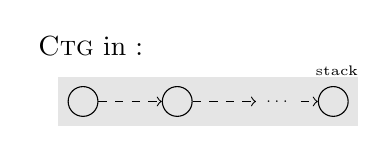
\begin{tikzpicture}
  [zstd/.style={state,font=\tiny},anchor=west]

  \draw (-0.5,1.2) node[anchor=west] (dummy){\ctg in :};
  \draw (0,0.5) node[zstd] (00) {};
  \draw (00)+(1,0) node[zstd] (01) {};
  \draw (01)+(1,0) node[font=\tiny,anchor=west] (02) {\dots};
  \draw (02)+(0.5,0) node[zstd] (03) {};
  \draw[dashed] (00) edge[->] (01)
    (01) edge[->] (02)
    (02) edge[->] (03);

    \begin{pgfonlayer}{background}
      \draw node[fit=(00) (03),fill=gray!20] (c1) {};
      \draw (c1.north east)
        node[anchor=south east,inner sep=0pt,font=\tiny]
        {stack};
    \end{pgfonlayer}
\end{tikzpicture}
\end{minipage}

    \caption{From a pushdown system  to a \qdas: \main and
     for  \label{fig:sim_pds}}
    \vspace{-4ex}
\end{figure}


The control state of the \pds is stored in the variable \texttt{state} and
the behaviour of the control structure of \Pp is encoded as non-determinstic
choice (line~) that assures that reaching the dispatch and termination actions
(lines~/) demands that the selected transition rule harmonizes with the
current change of the variable \texttt{state} from  to  and that a
 action is only possible if the currently running task is labeled
by the blockname  (line~).

A reachable configuration of 
is given by  where  is---as discussed before---a
path of vertices . As before, synchronous dispatch calls assure
there is no more than one task
active at the same time. Given 
and a configuration  that is reachable in ; then
 is represented by , written , iff
 and for 
 for  and . Hence, the state
of the \pds is stored in the variable \texttt{state}, and the path 
encodes in the underlying task's blocks the stack content, where the empty stack
is represented by a single vertex labeled by \main.

\begin{restatable}{proposition}{propsyncpdsqdas}
\label{prop:sync_pds_qdas}  Given a pushdown system , then we can generate  a
  synchronous \qdas  such that the following holds:
  for any
  run  in  there exists a
  run  of  such that
  for all 
  (),
  and vice versa.
\end{restatable}
\begin{proof}
  Given a run  of the \pds .
  W.l.o.g. let us consider in the following underlying sequence
  of configurations and fired transition rules
   where
   for .

  We show inductively how  generates a run that
  simulates .

  For the initial configuration of  
  and the initial configuration 
  with  consists of a single node  with
   and  it holds
  that .

  Now assert that the \pds  reached configuration  ()
  such that  simulated the prefix of the run until
   with
  . Assert that  is a path .
  We do a case-by-case analysis with respect
  to  that leads to :
  \begin{myitemize}
    \item only the task corresponding to  is active and
      the only way to exit its \texttt{while} loop is
      via the lines  and , that assure that line  selected
       with , and that we
      set ;;
    \item if  for , then
      we fire the synchronous dispatch that leads to  with , thus
      ;
    \item if  for  and we left the
      while loop then   (by line ), and
       equals , thus
      .
  \end{myitemize}

  The reverse direction follows analogously by considering lines 
  and  as atomic actions (i.e., setting the \texttt{state} variable
  and changing the call graph of the \qdas).
\end{proof}
\subsection{Asynchronous Concurrent \qdas}


\propfromqdastopn*

The proof of the proposition relies on the following lemma, showing
that  can simulate precisely the sequence of Parikh images that
are reachable in . Let  be a configuration of ,
and let  be marking of . We say that \emph{ encodes
  }, written  iff:  for all
: ,  for all : for all
:  and  for all  . Then:

\begin{lemma}\label{lemma:from-qdas-to-pn}
  Let  be a concurrent asynchronous \qdas with set of variables
   and set of locations , and let  be its associated
  \pn.  Then, for all  there is
   s.t.  and for all
  , there is  s.t. .
\end{lemma}
\begin{proof}
  We prove the two statements separately.

  Let  be a configuration in , and let
   be a
  run s.t. . Let us build, inductively, a run
   of  s.t. . The
  induction is on the length  of the \qdas run.

  \textbf{Base case .} It is easy to check that .

  \textbf{Inductive case .} Let us assume that  is a run of  s.t. ,
  and let us show how to complete it, if needed. We consider several
  case depending on . In the case where 
  and the scheduler action consists in dequeueing a block from a queue,
  we have  and
  . By induction hypothesis , hence ,
  and we do not add elements to the run built so far. In the case
  where , we assume
   is the corresponding \lts
  transition. Clearly,
  ,
  ,
   and
  for all other location :
  . It is easy to check
  that the \pn transition  s.t.  iff  and
   iff  is fireable from  (as
   by induction hypothesis) and
  yields the same effect, i.e. the marking  with
   is s.t. . All the
  other cases (test, assignment and task termination) are treated
  similarly.  \medskip

  Now, let  be a run of  and let us build,
  inductively, a run  s.t.  \emph{and} all
  the queues are empty in . The induction is on the length  of
  the \pn run.

  \textbf{Base case .} It is easy to check that .

  \textbf{Inductive case .} Let us assume that
   is a run of 
  s.t.  and all the queues are empty in
  . Let  be the \pn transition
  s.t.  and let us show how we can
  extend the run of . We consider several cases. If  is a
  transition that corresponds to an asynchronous dispatch, then there
  are , ,  and  s.t.  iff  and
   iff . By definition of ,
  there is a transition  in . Moreover,
  , since  is fireable from . As
  , the  is
  fireable from , and leads to a configuration
  , where a  block has been enqueued
  in , hence ,
  ,
  ,
   and for
  all other state : . It
  is easy to check that , however,
  queue  contains a call to  in  and is thus the
  only non-empty queue in this \ctg. Thus, from
  , we execute the scheduler action that
  dequeues from . This has no effect on the Parikh image of the
  \ctg. Thus, we reach 
  s.t. , ,
  hence  too, and all the queues are
  empty in , which concludes the induction step. All the
  other cases are treated similarly.\qed
\end{proof}


We can now prove Proposition~\ref{prop:from-qdas-to-pn}:
\begin{proof}
  It is easy to check that the construction of , as described
  above, is polynomial. Then, assume  is Parikh coverable in ,
  i.e. there is 
  s.t. . By Lemma~\ref{lemma:from-qdas-to-pn},
  there is  s.t. . Hence, for
  all : . So, for all :
  . Hence,  (as 
  for all ). Since , we conclude that
  . On the other hand, assume ,
  with  for all , and let  be s.t. for all
  : . Since , there is
   s.t. . By
  Lemma~\ref{lemma:from-qdas-to-pn}, there is
   s.t. . Thus, by
  definition of , for all : . Thus,
  since  and by definition of , we conclude that for all
  : . Hence,  is
  Parikh-coverable in .\qed
\end{proof}

\propfrompntoqdas*

The proof of Proposition~\ref{prop:from-pn-to-qdas} is split into two
lemmata, given hereunder. They rely on an alternate characterization of
. That is,  iff  is reachable by a
so-called \emph{lossy} run of , i.e. a sequence of markings
 s.t.  and for all : there is  and a transition 
s.t.  and
. Intuitively, a lossy run corresponds to
firing a transition of the PN, and then spontaneously losing some
tokens. The proof of these lemmata also assumes that each ,
the \lts  is as depicted in Fig.~\ref{fig:lts-p}.

\begin{figure}
  \centering
  \includegraphics[scale=.5]{lts-p}
  \caption{The \lts of bloc {\tt p}.}
  \label{fig:lts-p}
\end{figure}

\begin{lemma}
  Let  be a \pn, and let  be its corresponding \qdas.
  \textbf{If}  \textbf{then} there exists
   s.t. .
\end{lemma}
\begin{proof}
  Let  be a marking from .  and let 
  be a lossy \pn run s.t. . The proof is by induction on
  the length of the run. More precisely, we show that, for all , there is a reachable configuration
   s.t.: for all :
  , , ,  and
  .

  \textbf{Base case: }. Let us consider the run of  that
  consists in:  executing block \texttt{main} up to line 8, then
   emptying the queue . The execution of  has the effect
  that:  all  variables are initialized to  and keep this
  value,  for all place : \emph{at most}  copies of
  block \texttt{p} are asynchronously dispatched in queue  and
   one copy of block \texttt{trans} is dispatched in . Then,
  the execution of  creates one running task for each block that
  is present in . Thus, the execution of  followed by 
  reaches a configuration  with
   s.t.  (the queue has been emptied),
  for all : ,
   and
   (the queue is empty and all the calls are
  asynchronous). Moreover,  is such that each task running a
  \texttt{p} block is still in its initial state , hence
  . Similarly, the task running the \texttt{trans()}
  block is about to enter the \texttt{while} loop at line 14. Finally,
  as the variables have been initialized to  and not modified, we
  have  for all .

  \textbf{Inductive case: } Let us assume there exist
   that respects all the
  conditions given at the beginning of the proof (in particular
  ). Let  and  be the \pn transition
  and marking s.t. \smash{} and
   and let us show that  can simulate it. This
  is achieved by the following sequence of actions in . First,
  the block executing \texttt{trans} enters the \texttt{while} loop at
  line 14 and selects  as transition . Then, it sets all the
  variables  s.t.  to . Thus, at that point
   contains  iff , since all  variables
  were equal to  by induction hypothesis. Then, the task executing
  \texttt{trans} is blocked as it need to wait up to the point were
  all  are equal to . Since  by induction
  hypothesis, we know that there are, in ,  tasks
  executing block , for all . However,  is
  fireable from , and a loss of  token is still
  possible after the firing. Hence,  for all . Thus, for all ,
  there is at least  tasks executing
   in . Thus, we complete the run of  by
  letting, for all ,  \texttt{p}
  task execute lines 11 in turn one after the other. Then, letting
  them all execute line 12, and reach their final state (Remark that
  all the \texttt{p} task must first execute line 11 before one of
  them can execute line 12, as this sets  to  and would
  prevent other tasks to execute line 11). This is possible because
  none of those tasks are blocked, since the \ctg contains no edge, by
  induction hypothesis. At that point,  has reached a
  configuration  s.t.  for all 
  (by line 12) and where . Moreover,  still respects all
  the other hypothesis as no new dispatch have been performed. Then,
  the simulation of  proceeds by letting the \texttt{trans} task
  finish the current iteration of the main \texttt{while} loop. This
  consists in executing the \texttt{for} loop of line 19, which
  dispatches one \texttt{p} block in  iff , i.e., the
  effect of  is to add a token to . Finally, the scheduler
  empties queue  and creates tasks for all the blocks that have
  just been added to . It also kills all the \texttt{p} tasks that
  have reached their final state. As a consequence, the configuration
  that is reached is , where 
  and  is s.t.  for all . Moreover,
  since the queue has been emptied by the scheduler,  contains
  only task nodes and no edge, as all the calls are asynchronous. The
  task executing \texttt{trans} is still active and at line 14, and
  all the \texttt{p} tasks are in their initial state.\qed
\end{proof}

\begin{lemma}
  Let  be a \pn, and let  be its corresponding \qdas.
  \textbf{If} there are  and 
  s.t.  \textbf{then} .
\end{lemma}
\begin{proof}
  For a \ctg  of  with set of vertices , we denote by
   the marking of  s.t. for all : . Thus, in the case where  encodes a
  configuration s.t. \texttt{trans} is at line 14, \texttt{main} is at
  line 8, and all the \texttt{p} blocks are in their initial state,
  then .

  In order to establish the lemma, we prove a stronger statement:
  every time we reach, along a run, a configuration 
  s.t. \texttt{trans} is at line 14, then .
  Formally, let
  
  be a run of , where, for all :
  . Let
   be the monotonically
  increasing function s.t.  and for all :
  there exists  with  iff
  there is  with .  That is the
  sequence  identifies the indexes of
  all the configurations of the run where \texttt{trans} is at line
  14. Let us show, by induction on  that all the 's
  are reachable \emph{in the lossy semantics} of .

  \textbf{Base case } Let us show that , i.e.,
  that the first time \texttt{trans} reaches line 14, 
  is the initial marking of . Observe that the prefix of the run
  must have the following form. Initially, only the \texttt{main} block
  is executing: it first sets all the variables  to , then
  dispatches asynchronously at most  calls to each \texttt{p}
  block (for all ), then finally dispatches an asynchronous
  call to \texttt{trans} and reaches line 8. Along this execution, the
  scheduler might decide to pick up some \texttt{p} blocks from
  . However, as long as the scheduler has not scheduled the call to
  \texttt{trans}, the \ctg met along the run do not encode any
  marking, by definition of . When the scheduler starts a task
  to run the \texttt{trans} block, we thus reach a configuration
   where:  the queue  is empty, as dequeueing the
  \texttt{trans} block is possible only if all the \texttt{p} blocks
  have been dequeued, and no other dispatch has been performed; 
  all the \texttt{p} tasks are blocked in their initial state as
   for all ; and  \texttt{main} is still
  blocked in the infinite loop at line . Since the scheduler has
  just dequeued \texttt{trans} from ,  is necessarily the first
  \ctg to encode a marking, so . Moreover, by the loop
  at line 4, it is clear that  with .

  \textbf{Inductive case } The induction hypothesis is
  that . Let us consider the
  , i.e. the portion of  that allows to reach
   from
  . We consider two cases:
  \begin{enumerate}
  \item Either \textbf{trans} has not performed an iteration of its
    main \texttt{while} loop along . In this case, the only
    actions that can occur along  are scheduler actions
    consisting in dequeueing \texttt{p} blocks or the termination of
    some \texttt{p} tasks that where still in state . In
    both cases, this does not modify the value of , so
    .
  \item Or \texttt{trans} has performed a complete iteration of its
    main \texttt{while} loop possibly interleaved with the dequeue
    of \texttt{p} blocks and the termination of \texttt{p}
    tasks. Since the dequeues and terminations have no influence on
    the value of  as argued above, let us focus on the effect
    of executing one iteration of the \texttt{while} loop. The
    iteration first selects a \pn transition  and sets all the
    variables  s.t.  to . The reached configuration
    is then  where , as these
    operations do not manipulate \texttt{p} blocks or tasks. Then,
    \texttt{trans} is blocked by the test at line 18. As only
    \texttt{p} blocks can set  variables to , we are sure
    that, when \texttt{trans} reaches line 19, \emph{at least}
     \texttt{p} blocks have left their initial state, for all
    . Thus, when \texttt{trans} is at line 19, the
    configuration is , where for all :
    . Afterwards,
    \texttt{trans} terminates the iteration of the \texttt{while} loop
    by dispatching  \texttt{p} blocks for all , and
    reaches line 14, which finishes . Hence, we reach
    , where for all :
    . Since
     by induction hypothesis, we
    conclude that  too.\qed
  \end{enumerate}

\end{proof}




\subsection{Asynchronous Serial \qdas}
 We
establish the undecidability for asynchronous serial \qdas  by a reduction from the control-state  reachability
problem in a \fifo system. Let  be a
\fifo system and let  be a control state whose reachability
has to be tested. We build the asynchronous serial \qdas
 on domain , where ,
 and the  are
given by the pseudo code in Fig.~\ref{fig:fifo-to-qdas}.
\begin{figure}[t]
  \centering
    \begin{minipage}[t]{.45\linewidth}
      \begin{lstlisting}
global state, head
global s_queue q

def main():
  state := 
  head := 
  dispatch_a(q, )
  while(true): do nothing
      \end{lstlisting}

      \begin{minipage}{0.8\textwidth}
        \begin{tikzpicture}[overlay,remember picture]
          \draw node[anchor=north west,draw,
            rectangle callout,callout relative
            pointer={(1.2,-0.08)},font=\scriptsize, fill=gray!5,text
            width=4.7cm]
          {
      \scriptsize
      Note that the reachability of
      a state  of the \fifo system is explicitely coded
      into the control
      structure.};

        \end{tikzpicture}
    \end{minipage}

    \end{minipage}
    \begin{minipage}[t]{.5\linewidth}
      \begin{lstlisting}[firstnumber=last]
def m(): //for all 
  if (head): goto 20
  while(true):
    if (state = ): goto 21
    select 
    if (state): goto 20
    state := 
    if (): dispatch_a(q, )
    else if ():
      head := 
      terminate
  while(true): do nothing // wrong guess
  while(true): do nothing //  is reached
      \end{lstlisting}
    \end{minipage}

    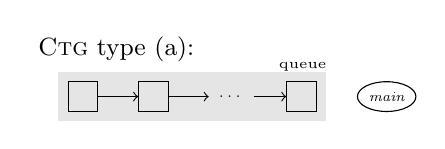
\begin{tikzpicture}
  [zstd/.style={state,font=\tiny},zstd2/.style={zstd,rectangle},anchor=west]

  \draw (-0.5,0.6) node[anchor=west] (dummy){\small \ctg type (a):};
  \draw (0,0) node[zstd2] (00) {};
  \draw (00)+(0.7,0) node[zstd2] (01) {};
  \draw (01)+(0.7,0) node[font=\tiny,anchor=west] (02) {\dots};
  \draw (02)+(0.7,0) node[zstd2] (03) {};
  \draw (03)+(0.7,0) node[zstd] (04) {\main};
  \draw (00) edge[->] (01)
    (01) edge[->] (02)
    (02) edge[->] (03);

    \begin{pgfonlayer}{background}
      \draw node[fit=(00) (03),fill=gray!20] (c1) {};
      \draw (c1.north east)
        node[anchor=south east,inner sep=0pt,font=\tiny]
        {queue };
    \end{pgfonlayer}
  \end{tikzpicture}\hspace{1cm}
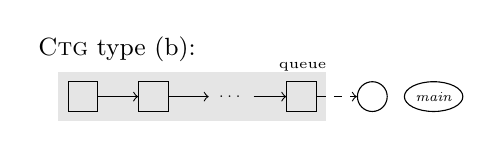
\begin{tikzpicture}
  [zstd/.style={state,font=\tiny},zstd2/.style={zstd,rectangle},anchor=west]

  \draw (-0.5,0.6) node[anchor=west] (dummy){\small \ctg type (b):};
  \draw (0,0) node[zstd2] (00) {};
  \draw (00)+(0.7,0) node[zstd2] (01) {};
  \draw (01)+(0.7,0) node[font=\tiny,anchor=west] (02) {\dots};
  \draw (02)+(0.7,0) node[zstd2] (03) {};
  \draw (03)+(0.7,0) node[zstd] (04) {};
  \draw (04)+(0.4,0) node[zstd] (05) {\main};
  \draw (00) edge[->] (01)
    (01) edge[->] (02)
    (02) edge[->] (03)
    (03) edge[->,dashed] (04);

    \begin{pgfonlayer}{background}
      \draw node[fit=(00) (03),fill=gray!20] (c1) {};
      \draw (c1.north east)
        node[anchor=south east,inner sep=0pt,font=\tiny]
        {queue };
    \end{pgfonlayer}
\end{tikzpicture}
    \caption{Fifo system encoding into a serial asynchronous
      \qdas / two types of \ctg in this case}
  \label{fig:fifo-to-qdas}
  \label{fig:shapes-aaf}
\vspace{-2ex}
\end{figure}


Intuitively, runs of  simulate the runs of , by encoding the
current state of  in variable \texttt{state} and the content of
's queue into the content of the serial queue \texttt{q}. More
precisely, it easy to check that, once \texttt{main} has reached
line~8, all the \ctg that are reached in  are of either shapes
depicted in Fig.~\ref{fig:shapes-aaf}, for . That is, there are at most two running
tasks: \texttt{main} and possibly one task running a  block (for
), that has to terminate to allow a further
dequeue from \texttt{q}. This is because \texttt{q} is a serial queue
and all the dispatches are asynchronous. When the \ctg is of shape
\textsf{(b)}, the duty of the running  block is to simulate a run
of . It runs an infinite \texttt{while} loop (line 11 onwards --
ignore the test at line 10 for the moment), that  tests whether
 has been reached (line 12) and jumps to line 20 if it is the case;
 guesses a transition  of ; and  checks that
the guessed transition is indeed fireable from the current
configuration of , and, if yes, simulate it. This consists in,
first testing that  is the current state (line 14). If not, the
block jumps to the infinite loop of line 19, which ends the
simulation. Otherwise, the current state is update to , and the
channel operation is then simulated. A send of message  is
simulated (line 16) by an asynchronous dispatch of block  to
\texttt{q}. The simulation of a receive of  from \texttt{q} is more
involved, as only the scheduler can decide to dequeue a block from
\texttt{q}, and this can happen only if the current running block
terminates (line 19). Still, we have to check that message  is
indeed in the head of \texttt{q}. This is achieved by setting global
variable \texttt{head} to , and letting the next dequeues block
check that itself encodes the value stored into \texttt{head}. This is
performed at line 10. If this test is not satisfied, the block jumps
to the infinite loop of line 20, and the simulation ends. Otherwise,
it proceeds with the simulation. Thus, in all reachable configurations
of , a block  (with  will reach line 21
iff  is reachable in . This effectively reduces the control
location reachability of \fifo systems to the Parikh coverability
problem of serial asynchronous \qdas.


The proof of Theorem~\ref{the:async-seri-undec} relies on the
next Lemma, that formalizes the relationship between reachable
configurations of  and reachable configurations of~.

For all , we denote by  the
location of  that corresponds to line  in
Fig.~\ref{fig:fifo-to-qdas}. Then, we say that a configuration
 of  encodes a configuration  of ,
written  iff: 
,   is of either shapes in
Fig.~\ref{fig:shapes-aaf} with , 
 and  there exists  s.t. . That is,  and
 are encoded as described above, \texttt{main} is at line 8, and
the running  block is at line 12. Then:

\begin{lemma}\label{lem:from-fifo-to-qdas}
  Let  be a FIFO system, let  be a configuration of , and let
   be its associated \qdas. For all run
   of  s.t. for all :
  , there exists  s.t.
  . Moreover, for all
   and for all configuration  of
  :  implies 
\end{lemma}
\begin{proof}
  First, we consider a run  of 
  s.t. for all : , and build a run
   of 
  s.t. , by induction on the length
  of 's run.

  \textbf{Base case :} Consider the run of  that consists
  in executing lines 5, 6, 7 of \texttt{main} (which sets the
  \texttt{head} variable to ), then dequeueing the  block from
  the queue, then executing lines 10 and 11 of . Remark that the
  test at line 10 is not satisfied, as , and that
  the queue is now empty. Clearly, the resulting configuration
   as .

  \textbf{Inductive case }. Let us assume that there is a
  reachable configuration  of 
  s.t. , and let us build
  a sequence of  transitions that is fireable from
   and reaches a configuration encoding
  . In , there is, by definition of
  , a task running a  block, for , that is
  at line 12. Moreover, . Let
   be the transition of 
  s.t. . By
  hypothesis, , hence, we let  execute line 12;
  select  at line 13; execute line 14,
  where the condition of the \texttt{if} is not satisfied as
  ; and execute line 16, which reaches a
  configuration  where
  . We consider three cases to complete
  the simulation of  in . If , the  task
  performs an asynchronous dispatch of  to \texttt{q}, and jumps to
  line 11, then 12. Clearly, the resulting configuration
   is s.t. 
  (in particular, the dispatch has correctly updated the content of
  the queue). If , the  tasks jumps directly to line 11, then
  to line 12. Again, the resulting configuration 
  is s.t. , as the content of
  the queue has not been modified. Finally, if , the running 
  block sets \texttt{head} to  and terminates. Let
   be the  configuration reached at that
  point. As  is fireable from  in ,
  since , and as the
  content of the queue has not been modified since then, the head of
  \texttt{q} is necessarily an  block in . Moreover,
   and
  . Thus, we let the scheduler dequeue
  this  block, and we let the task running it execute line 10
  (where the condition of the \texttt{if} is not satisfied), then line
  11. Clearly, the resulting configuration encodes .
  \medskip

  Now, let  be a run of  s.t. there is  with
  , and let us build, by induction on the
  length of this run, a run  a
  run of  s.t. .

  Let
  , i.e.,  is the number of times an
   block reaches line  along . Let us consider the
  increasing monotonic function
   s.t. for all : there exists 
  s.t.  iff there is  s.t. , that is,  is the index,
  in  of the th time a configuration is reached where an
   block is at line 12. Clearly, by definition of 
  only the  configurations (for
  ) can encode a configuration of , as no  block
  is at line 12 in the other configurations of . So, it is
  sufficient to show that all those
   configurations encode a
  reachable configuration of . We proceed by induction on , and
  show that: for all :
   encodes a reachable
  configuration of  and  contains exactly one 
  task (for ), that has been dequeued from
  \texttt{q}.

  \textbf{Base case :} Observe that the subrun
   is necessarily an
  initialization phase where \texttt{main} sets \texttt{state} to
  , \texttt{head} to , dispatches an  block, and
  reaches line 8, where it will stay forever. Then, the scheduler
  dequeues the  block, which empties the queue. The  task then
  traverses line 10 (as \texttt{head}) and 11 and reaches line
  12. So, clearly 
  and contains exactly one  task (for ), that has
  been dequeued from \texttt{q}.


  \textbf{Inductive case :} Let us assume that
   encodes a reachable
  configuration  of . We consider several
  cases. If  we are done. Otherwise, we
  have necessarily performed one iteration (possibly interrupted at
  line 12, 14 or 19) of the while loop at line 11 between
   and
  , as, by induction
  hypothesis,  contains exactly one  task
  (with ) that blocks \texttt{q}, and \texttt{main}
  can only loop at line 8, which does not modify the current
  configuration. Then, observe that the conditions of the \texttt{if}
  at lines 12 and 14 were necessarily false during the
  iteration. Otherwise,  would have reached line 21, from which it
  cannot escape. From that point, no configuration is reachable where
  an  block is at line 12 , and  cannot exist.  Thus, we consider three cases:
  \begin{itemize}
  \item If we have entered the \texttt{if} at line 16 during the
    iteration, then a transition of the form  has been
    guessed, with  and a dispatch of  has been
    performed into . As
     by induction hypothesis, , and thus
     is fireable from  and reaches
    . Clearly, this configuration is encoded
    by .
  \item If we have entered the \texttt{else if} at line 17 during the
    iteration, then a transition of the form  has been
    guessed, with , \texttt{head} has been set to
    , the current  block has been terminated, a new block 
    has been dequeued by the scheduler (as there is necessarily a
    running \texttt{m} block in ). Moreover
    , because  has to be at line 12 in
    , so the test of line 10 had to be false to
    allow  to reach line 12. As
     by induction hypothesis, . As a dequeue
    of a block  has been performed,  is of the form
    . Thus,  is fireable from  and reaches . Clearly, this configuration is
    encoded by .
  \item Finally, if neither the \texttt{if} nor the \texttt{else if}
    have been entered during the iteration, then a transition of the
    form  has been guessed, with . As
     by induction hypothesis, , and thus
     is fireable from  and reaches
    . Clearly, this configuration is encoded by
    .\qed
  \end{itemize}
\end{proof}



We can now prove Theorem~\ref{the:async-seri-undec}:
\begin{proof}
  Let  be a FIFO system, with set of messages  and associated
  serial asynchronous \qdas  and let  be a control location
  of . For all , let  be the Parikh image
  s.t.  and  for all . Remark that there are only finitely many
  such . Then, we show that  is reachable in  iff there
  exists  s.t.   is Parikh-coverable in
  .

  Assume  is reachable in , and let  be a configuration
  in . Without loss of generality, assume  is reachable
  by run that visits  only once. By
  Lemma~\ref{lem:from-fifo-to-qdas}, there is
  
  s.t. . Hence, in , there is
  a task running an  block (for ) that is at line
  12, and . Thus,  can execute one step
  and reach line 21, so  is Parikh coverable in .

  For the reverse direction, assume there is  that
  is Parikh-coverable in . Hence, there is
   where a task running block  is
  at line 21. The only way for that block to reach line 21 is from
  line 12, with a valuation 
  s.t. . Thus, there is, in 
  a configuration  with ,
  a task running an  block at line 12, and necessarily
  \texttt{main} at line 8 (otherwise, only \texttt{main} would be
  running). Hence,  is a reachable configuration of
   s.t.  for some queue content
  . Thus, by Lemma~\ref{lem:from-fifo-to-qdas},
  , and  is reachable in .

  We have thus reduced the control location reachability problem of
  FIFO systems to the Parikh coverability problem of serial
  asynchronous \qdas (using only one serial queue). The former is
  undecidable. Hence the theorem.\qed
\end{proof}


\subsection{Concurrent \qdas}

We reduce the reachability problem of two counter
systems. Let us give the intuition of the construction. For each
, we construct a \qdas  s.t. all reachable \ctg in
 encode configurations of  and are of the form depicted
in Fig.\,\ref{fig:sim_counter}. That is, (after an initialization
phase), there are always three tasks that are unblocked: a \main task
to simulate 's control structure, and, for each ,
either a task  or a task . If the task  is
unblocked, then counter  is zero in the current configuration of
. Otherwise, the current valuation of counter  is encoded by
the number of  tasks in the \ctg. Remark that, as in the case
of synchronous \qdas, the parts of the \ctg that encode each counter
behave as pushdown stacks. Finally, the control location of  is recorded in
global variable \texttt{state}.

\begin{figure}[t!]
  \centering
  \begin{minipage}[t]{.5\linewidth}
      \begin{lstlisting}
global state
global , ,  // rdvz channel 1
global , ,  // rdvz channel 2
global c_queue q

def main():
  foreach i in {1,2}:
    dispatch_a(q, null(i))
    i?ack
  state := 

  while(true):
    select  where state=

    if  :
      1!
      1?
      state:=

    \\ other actions analogous
    ...
      \end{lstlisting}
    \end{minipage}
    \begin{minipage}[t]{.5\linewidth}
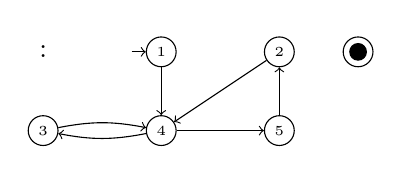
\begin{tikzpicture}[baseline=(base),
  zstd/.style={state,font=\tiny}]
  \draw (0,0.3) coordinate (base);
  \draw (1.5,0) node[zstd] (1) {{1}};
  \draw (1)+(-0.5,0) node (s) {}
      (s) edge[->] (1);
  \draw (3,0) node[zstd] (2) {2};
  \draw (4,0) node[zstd] (f) {};
  \draw[fill=black] (f) circle (3pt);
  \draw (0,-1) node[zstd] (3) {3};
  \draw (1.5,-1) node[zstd] (4) {4};
  \draw (3,-1) node[zstd] (5) {5};
  \draw (3) edge[->,bend left=11] node[above,font=\tiny]{} (4);
  \draw (4) edge[->,bend left=11] node[below,font=\tiny]{} (3);
  \draw (1) edge[->] node[left,font=\tiny,pos=0.3]{} (4);
  \draw (4) edge[->] node[below,font=\tiny]{}(5);
  \draw (5) edge[->] node[right,font=\tiny]{} (2);
  \draw (2) edge[->] node[left,pos=0.3,font=\tiny]{\ }(4);

  \draw (0,0) node {:};
\end{tikzpicture}

\vspace{2ex}
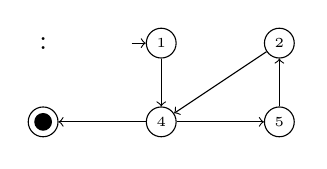
\begin{tikzpicture}
  [zstd/.style={state,font=\tiny}]
  \draw (1.5,0) node[zstd] (1) {1};
  \draw (1)+(-0.5,0) node (s) {}
      (s) edge[->] (1);
  \draw (3,0) node[zstd] (2) {2};
  \draw (0,-1) node[zstd] (3) {};
  \draw[fill=black] (3) circle (3pt);
  \draw (1.5,-1) node[zstd] (4) {4};
  \draw (3,-1) node[zstd] (5) {5};
  \draw (4) edge[->] node[below,font=\tiny]{} (3);
  \draw (1) edge[->] node[left,font=\tiny,pos=0.3]{} (4);
  \draw (4) edge[->] node[below,font=\tiny]{}(5);
  \draw (5) edge[->] node[right,font=\tiny]{} (2);
  \draw (2) edge[->] node[left,pos=0.3,font=\tiny]{\ }(4);

  \draw (0,0) node {:};
\end{tikzpicture}

\vspace{2ex}
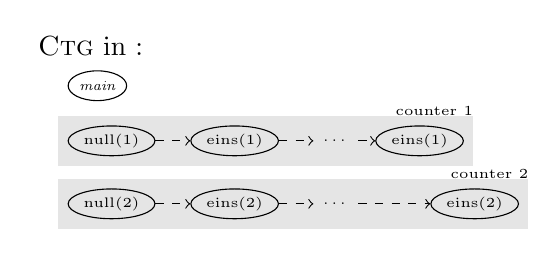
\begin{tikzpicture}
  [zstd/.style={state,font=\tiny},anchor=west]

  \draw (-0.5,1.2) node[anchor=west] (dummy){\ctg in :};
  \draw (0,0.7) node[zstd] (0) {\main};
  \draw (0,0) node[zstd] (00) {null(1)};
  \draw (00)+(1,0) node[zstd] (01) {eins(1)};
  \draw (01)+(1,0) node[font=\tiny,anchor=west] (02) {\dots};
  \draw (02)+(0.5,0) node[zstd] (03) {eins(1)};
  \draw (0,-0.8) node[zstd] (11) {null(2)};
  \draw (11)+(1,0) node[zstd] (12) {eins(2)};
  \draw (12)+(1,0) node[font=\tiny,anchor=west] (13) {\dots};
  \draw (13)+(1.2,0) node[zstd] (14) {eins(2)};
  \draw[dashed] (00) edge[->] (01)
    (01) edge[->] (02)
    (02) edge[->] (03)
    (11) edge[->] (12)
    (12) edge[->] (13)
    (13) edge[->] (14);

    \begin{pgfonlayer}{background}
      \draw node[fit=(00) (03),fill=gray!20] (c1) {};
      \draw node[fit=(11) (14),fill=gray!20] (c2){};
      \draw (c1.north east)
        node[anchor=south east,inner sep=0pt,font=\tiny]
        {counter 1};
      \draw (c2.north east)
        node[anchor=south east,inner sep=0pt,font=\tiny]
        {counter 2};
    \end{pgfonlayer}
\end{tikzpicture}
    \end{minipage}

    \caption{From a two counter system  to a \qdas: \main and
     for  \label{fig:sim_counter}}
    \vspace{-4ex}
\end{figure}

The actual operations on the counters will be simulated by the
 and  running tasks. As \main simulates the control
structure, we need to synchronize
\main with those  and  tasks.  Let us explain
intuitively how we can achieve \emph{rendezvous} synchronization
between running tasks using global variables of \qdas. Consider a
\qdas with three global variables ,  ranging over
Boolean and  over a finite set of `messages' .
Let  and  be two blocks whose \lts
are:\\
: 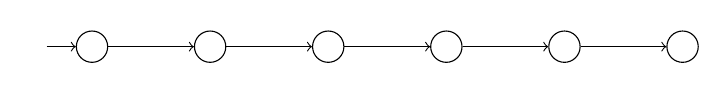
\begin{tikzpicture}[baseline=-0.5ex] \foreach \x in
  {0,1,2,3,4,5} \draw (1.5*\x,0) node[circle,draw,inner sep=4pt] (\x)
  {}; \draw (0) node[font=\tiny]{}; \draw (5)
  node[font=\tiny]{}; \draw (0) edge[->]
  node[above,font=\tiny]{} (1); \draw (1) edge[->]
  node[above,font=\tiny]{} (2); \draw (2) edge[->]
  node[above,font=\tiny]{} (3); \draw (3) edge[->]
  node[above,font=\tiny]{} (4); \draw (4) edge[->]
  node[above,font=\tiny]{} (5); \draw (0)+(-0.7,0) node
  (z) {} (z) edge[->](0);
\end{tikzpicture}\hfill (for )\\
: 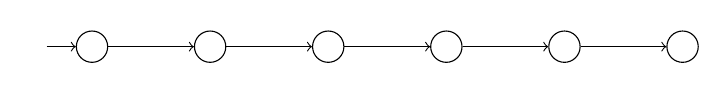
\begin{tikzpicture}[baseline=-0.5ex]
  \foreach \x in {0,1,2,3,4,5}
  \draw (1.5*\x,0) node[circle,draw,inner sep=4pt] (\x) {};
  \draw (0) node[font=\tiny]{};
  \draw (5) node[font=\tiny]{};
  \draw (0) edge[->] node[above,font=\tiny]{} (1);
  \draw (1) edge[->] node[above,font=\tiny]{} (2);
  \draw (2) edge[->] node[above,font=\tiny]{} (3);
  \draw (3) edge[->] node[above,font=\tiny]{} (4);
  \draw (4) edge[->] node[above,font=\tiny]{} (5);
  \draw (0)+(-0.7,0) node (z) {} (z) edge[->](0);
\end{tikzpicture}\\
Assume a configuration  of the \qdas where  and
where two distinct tasks are running  and , are
unblocked, and are in  and  respectively.  Assume that no
other task can access ,  and . It is easy to check
that, from , there is only one possible interleaving of the transitions
of and . So if  reaches  from ,
then  must have reached , and the  test in
 has been fired \emph{after} the  assignment in
. This achieves rendezvous synchronisation between
 and , with the passing of message . This can
easily be extended to rendezvous via different ``channels'', by adding
extra global variables. So, we extend the syntax of
\qdas by allowing transitions of the form  and
 (for ) to denote respectively a send and a
receive of message  on a rendezvous channel .



We rely on this mechanism to let \main send operations to be performed
on the counters to the  and  running tasks. More
precisely, for a \twocs , we
build the \qdas  where ,
,
 where 
range over the domain , and the
transition systems are given in Fig.\,\ref{fig:sim_counter}. The
variables  encode two channels that we call  and  in the
pseudo code of Fig.~\ref{fig:sim_counter}. The \main task runs an
infinite \texttt{while} loop (line 12 onwards) that consists in
guessing a transition  of  and synchronising, via
\emph{rendezvous} on the channels  and , with the relevant
 or  unblocked task, to let it execute the operation on
the counter. When a  or  receives an 
message, it performs an asynchronous dispatch of  into  to
increment counter , and acknowledges the operation to \main, thanks
to message . When an  block receives a  message, it
terminates, which decrements the counter.  blocks cannot receive
 messages, so, if \main requests a  operation when the
counter is zero, \main gets blocked. This means that the guessed
transition was not fireable in the currently simulated \twocs configuration, and ends the
simulation. Finally, only  blocks can receive and acknowledge
 messages, so, again, \main is blocked after sending
 to a non-zero counter.
Note that we need both \emph{asynchronous} calls to start two counters
in parallel, and \emph{synchronous} calls to encode the counter
values. The result of Theorem\,\ref{thm:concqdasundec} follows
directly from:

\begin{restatable}{proposition}{propsimpdsrdvzqdas}
  \label{prop:sim_pds_rdvz_qdas}
  Given a \twocs,
  then we can reduce its reachability question
  to the Parikh coverability question for a concurrent \qdas that demands
  both synchronous and asynchronous dispatch actions.
\end{restatable}


As discussed before, we can separate each  for
 into three components, one
consisting only of a vertex  with 
and two paths  and  which
we will call  and  in the following.

As before, we define a relation between configurations of the \twocs  and
the \qdas . For  and
 we
write  if , ,
and .

The rendezvous assures a unique interleaving of actions of \main, ,
and  until \main reaches line . Let us in the following consider
the reached configuration  with ,
 and
 with\\

\begin{tikzpicture}
  [zstd/.style={state,font=\small,inner sep=1pt,minimum size=15pt},
  zstd2/.style={zstd,rectangle},
  lab/.style={font=\tiny,inner sep=1pt},
  anchor=west]
    \draw  node[zstd] (13) {};
    \draw (13.south east) node[lab,anchor=north west] {};
    \draw (13.north east) node[lab,anchor=south west] {};

    \draw (1.5,0) node[zstd] (13) {};
    \draw (13.south east) node[lab,anchor=north west] {};
    \draw (13.north east) node[lab,anchor=south west] {};

    \draw (3.5,0) node[zstd] (13) {};
    \draw (13.south east) node[lab,anchor=north west] {};
    \draw (13.north east) node[lab,anchor=south west] {};
\end{tikzpicture}\\
(where  is the state of \main in line ) as ``initial'' configuration of the \qdas.

Note that  and  are independent, i.e., they do not
synchronize except via . Further, there is no more than one task active
in  and . The unique tasks  and 
never terminate. The rendezvous synchronization assures that there is only
\emph{one} possible interleaving between the \main task and the currently running
tasks in  and :
\begin{myitemize}
  \item \main does loops of the form\\
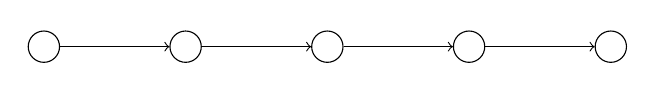
\begin{tikzpicture}[baseline=-0.5ex]
  \foreach \x in {0,1,2,3,4}
    \draw (1.8*\x,0) node[circle,draw,inner sep=4pt] (\x) {};

  \draw (0) node[font=\tiny]{};
  \draw (4) node[font=\tiny]{};
  \draw (0) edge[->] node[above,font=\tiny]{} (1);
  \draw (1) edge[->] node[above,font=\tiny]{} (2);
  \draw (2) edge[->] node[above,font=\tiny]{} (3);
  \draw (3) edge[->] node[above,font=\tiny]{} (4);
\end{tikzpicture}\hfill (for )\\

  \item which leads to the following interleaving of actions of \main
    with actions of the -th counter component.\\
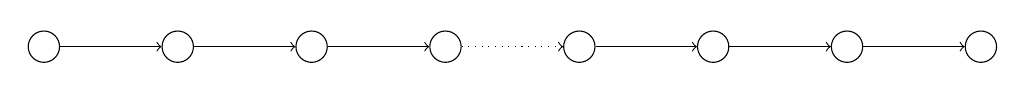
\begin{tikzpicture}
  \foreach \x in {0,1,2,3,4,5,6,7}
    \draw (1.7*\x,0) node[circle,draw,inner sep=4pt] (\x) {};

  \draw (0) edge[->] node[above,font=\tiny]{} (1);
  \draw (1) edge[->] node[above,font=\tiny]{} (2);
  \draw (2) edge[->] node[above,font=\tiny]{} (3);
  \draw (3) edge[->,dotted] node[above,font=\tiny]{} (4);
  \draw (4) edge[->] node[above,font=\tiny]{} (5);
  \draw (5) edge[->] node[above,font=\tiny]{} (6);
  \draw (6) edge[->] node[above,font=\tiny]{} (7);
\end{tikzpicture}\\

where
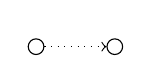
\begin{tikzpicture}
  \draw node[circle,draw,inner sep=2pt] (a) {};
  \draw +(1,0) node[circle,draw,inner sep=2pt] (b) {};
  \draw (a) edge[->,dotted] node[above,font=\tiny]{} (b);
\end{tikzpicture}
translates the sent action  to a meta-action  of the -th counter
as follows:\\
\begin{myitemize}
  \item an action  is mapped to the action
     and the activation of the dispatched task
  \item an action  is mapped to the termination of
    the current task; which is only possible if the current task
    is a block 
  \item the test for empty stack is mapped to an epsilon action; this action
    is only possible in .
\end{myitemize}
\end{myitemize}
Note that if  is not possible, then there will be no acknowledgement,
hence  blocks.

Thus we can cut a run of  into (an initial phase and) a sequence of
phases of the above form that will be abbreviated  in the
following.


\begin{lemma}
  Let  be a \twocs and 
  the associated \qdas, if   then there exists
   such
  that . Further, if 
  where  valuates ,
  then there exists  with .
\end{lemma}

\begin{proof}

  Given a run  of
  , then there exists a run of  that can be cut into
  phases  where  where
   for .
    Obviously  and
  .
  Hence, the reverse direction follows by a straightforward inductive
  argument.
      \end{proof}









\end{document}
